\documentclass[parskip=full]{scrartcl}
\usepackage[utf8]{inputenc}
\usepackage[T1]{fontenc}
\usepackage[ngerman]{babel}
\usepackage{enumerate}
\usepackage{enumitem}
\usepackage{hyperref}
\usepackage{graphicx}
\usepackage{float}
\usepackage{lmodern}
\usepackage{csquotes}
%\usepackage[toc]{glossaries}

\setlist[enumerate]{itemsep=-2.5mm}
\setlist[enumerate,2]{label=\arabic*.}
\setlist[description]{itemsep=-2.5mm}
\newcommand{\req}[1]{\mbox{/#1/}}

\title{ContentBasedBrowser -CoBaB- \\ Entwurfsdokument}
\hypersetup{
    colorlinks,
    citecolor=black,
    filecolor=black,
    linkcolor=black,
    urlcolor=black
}

%\renewcommand{\glossarysection}[2][]{}
%\makeglossaries


\begin{document}
\begin{titlepage}
\title{ContentBasedBrowser -CoBaB- \\ Entwurf}
\author{Anja Blechinger, Marie Bommersheim, Georgi Georgiev,\\ Tung Nguyen, Vincent Winkler, Violina Zhekova}
\date{Dezember 2015}
\maketitle
\vspace{300pt}
\begin{tabular}{l l}
Projekt: & Media Browser zur inhaltsbasierten Suche in Bild- und Videodaten\\
Auftraggeber: & Arne Schumann,\\
 & Fraunhofer Institut für Optronik, Systemtechnik und Bildauswertung,\\
 & Karlsruhe\\
\end{tabular}
\thispagestyle{empty}
\end{titlepage}
\setcounter{page}{1}

\tableofcontents

\section{Einleitung}
In diesem Dokument wird die Qualitätssicherung von CoBaB beschrieben. \newline
Die Aufgabe dieser Phase ist es, die Bedienbarkeit und Funktionalität von CoBaB zu testen und eventuelle Fehler zu beheben. Dies ermöglichen die im Pflichtenheft beschriebenen und weitere Testszenarien. \newline
Außerdem wird überprüft, wie viel des erarbeiteten Codes durch die Testfälle abgedeckt wird. 

\section{Aufbau}
\subsection{Architektur}

\begin{figure}[H]
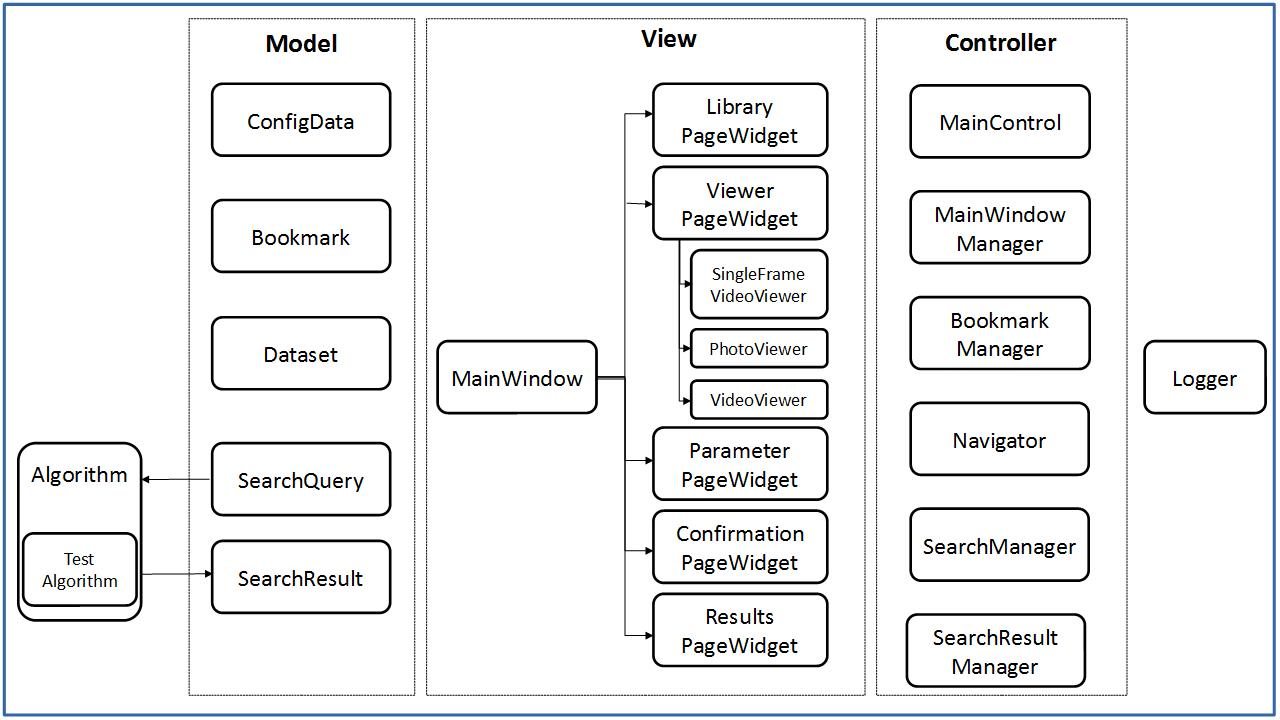
\includegraphics[width=1\linewidth]{img/architektur}
\caption{Architektur}
\label{fig:architektur}
\end{figure}

\subsection{Klassendiagramm}

\begin{figure}[H]
	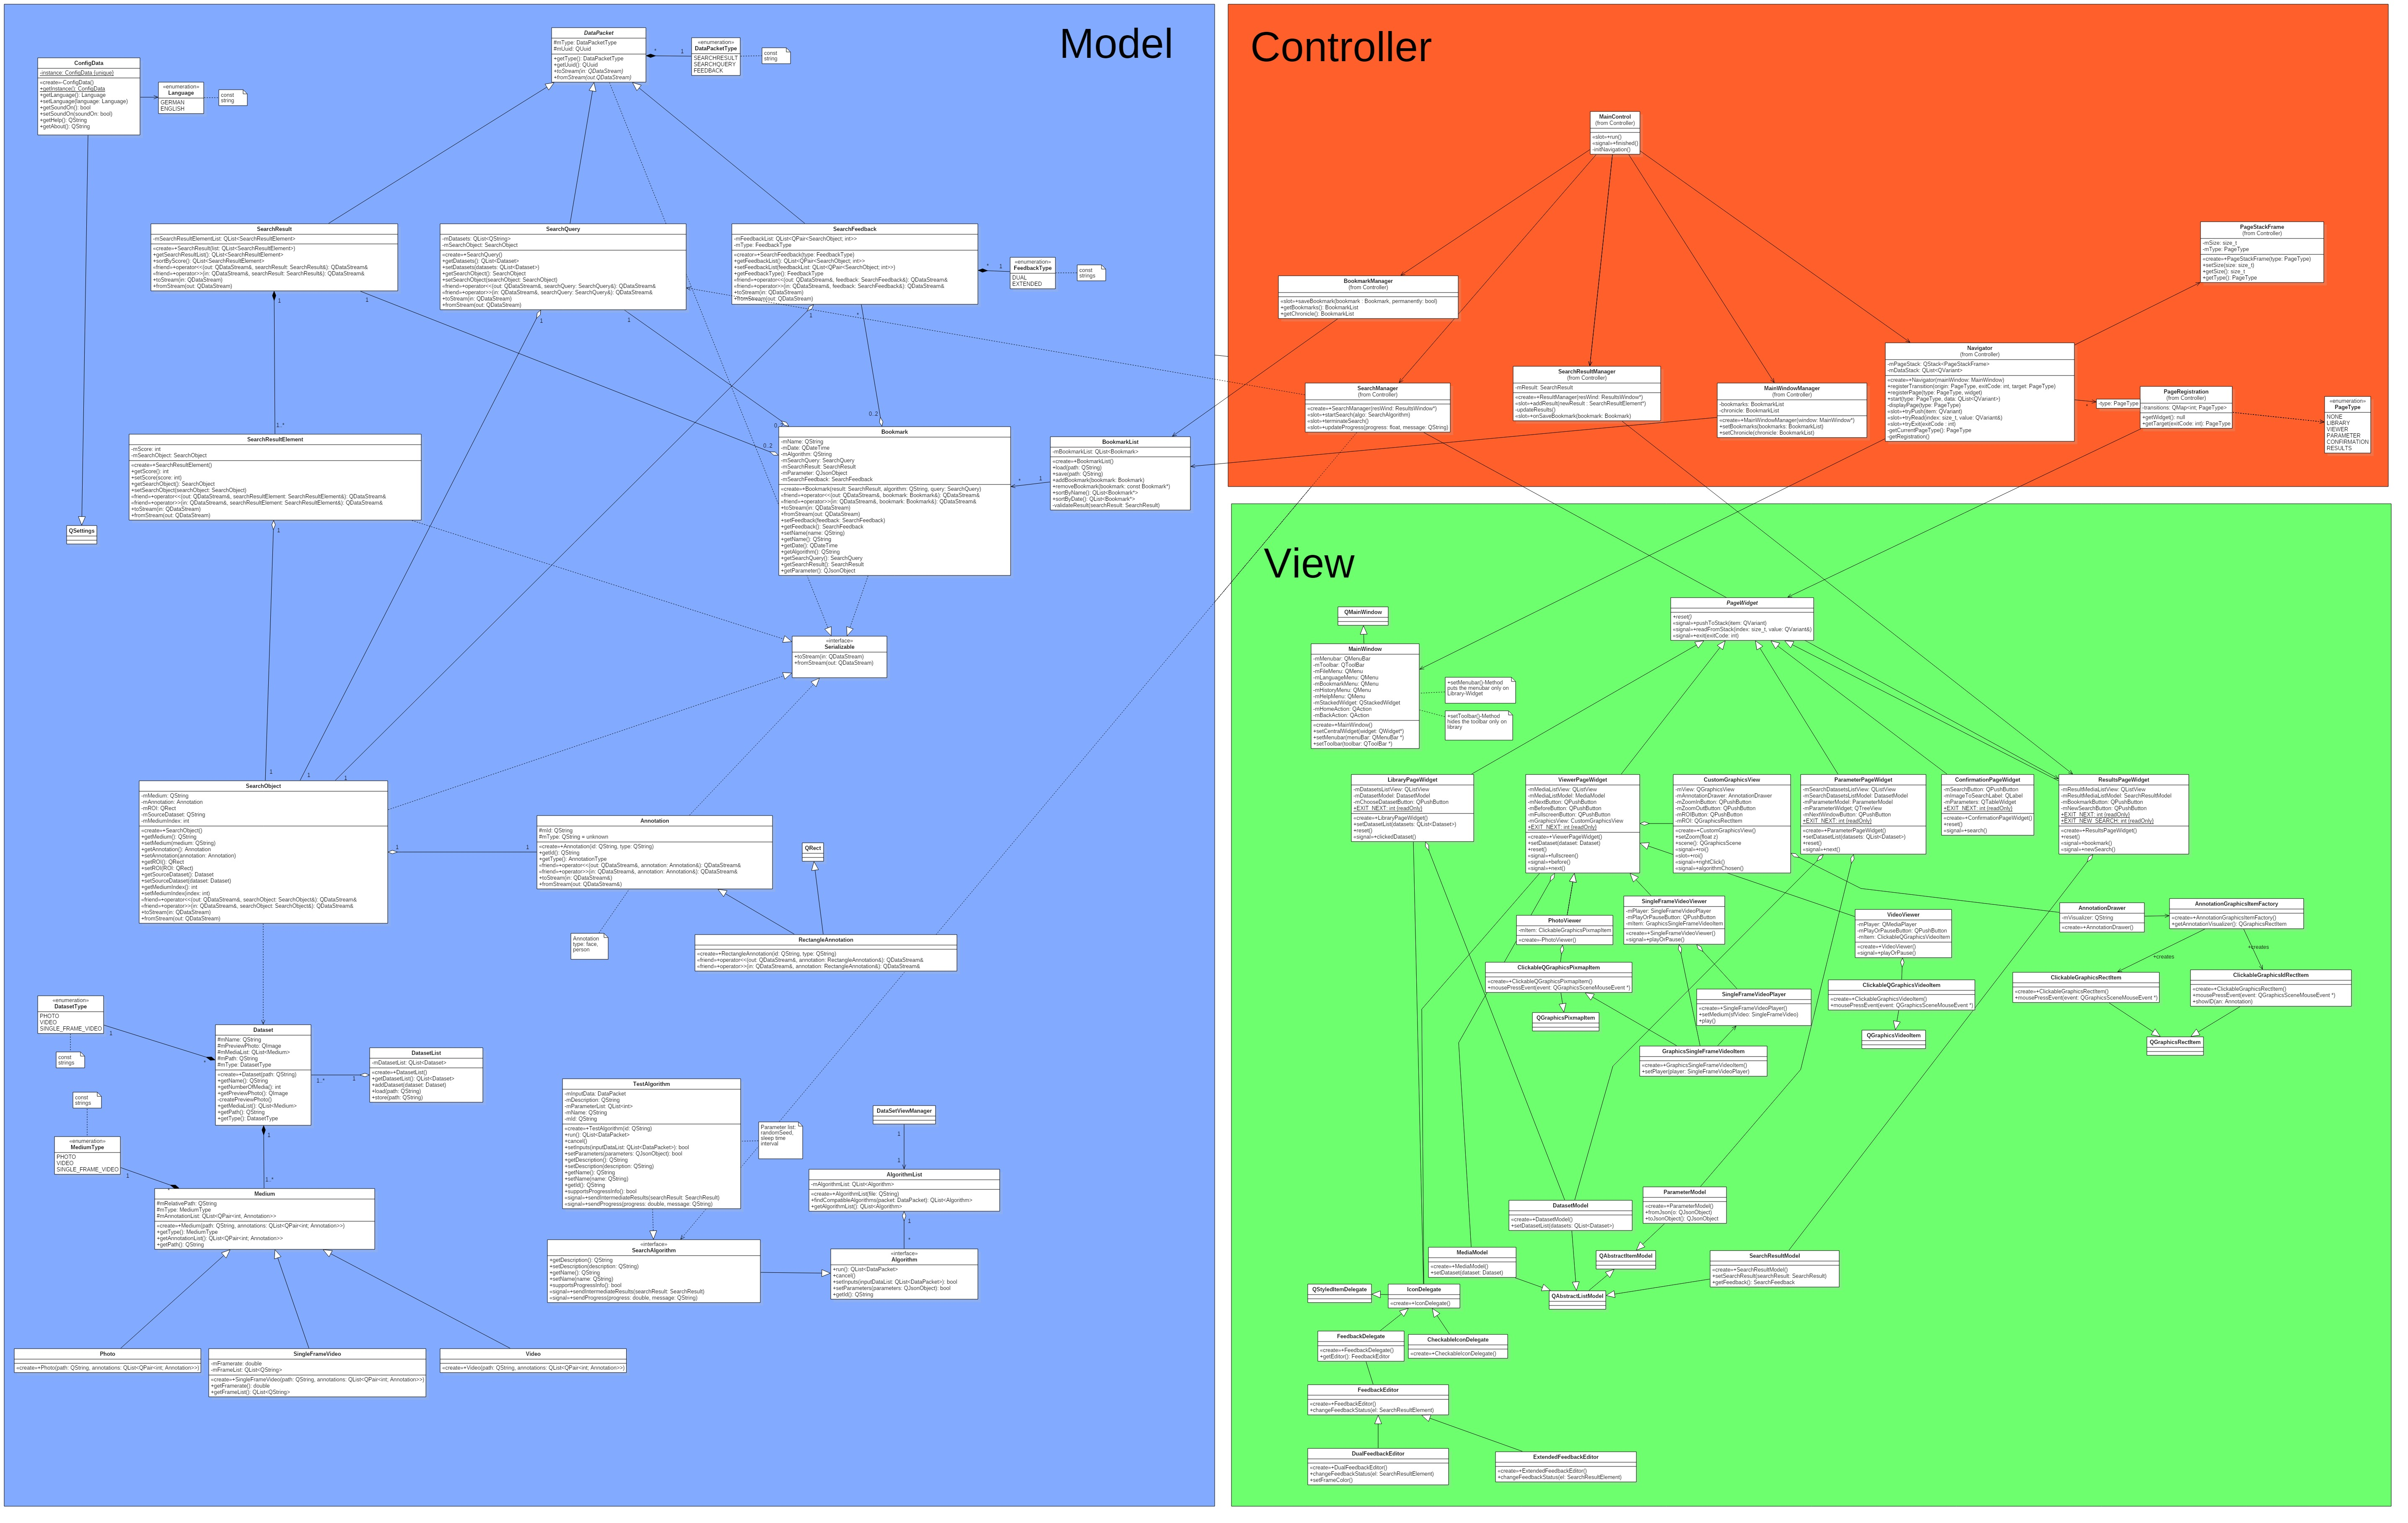
\includegraphics[width=1\linewidth]{img/Klassendiagramm/Complete}
	\caption{Klassendiagramm}
	\label{fig:klassendiagramm}
\end{figure}



\section{Klassenbeschreibung}
\subsection{Model}
Dieses Diagramm zeigt alle Klassen des Models. Die zugehörigen Attribute und Methoden werden im Folgenden beschrieben.

\begin{figure}[H]
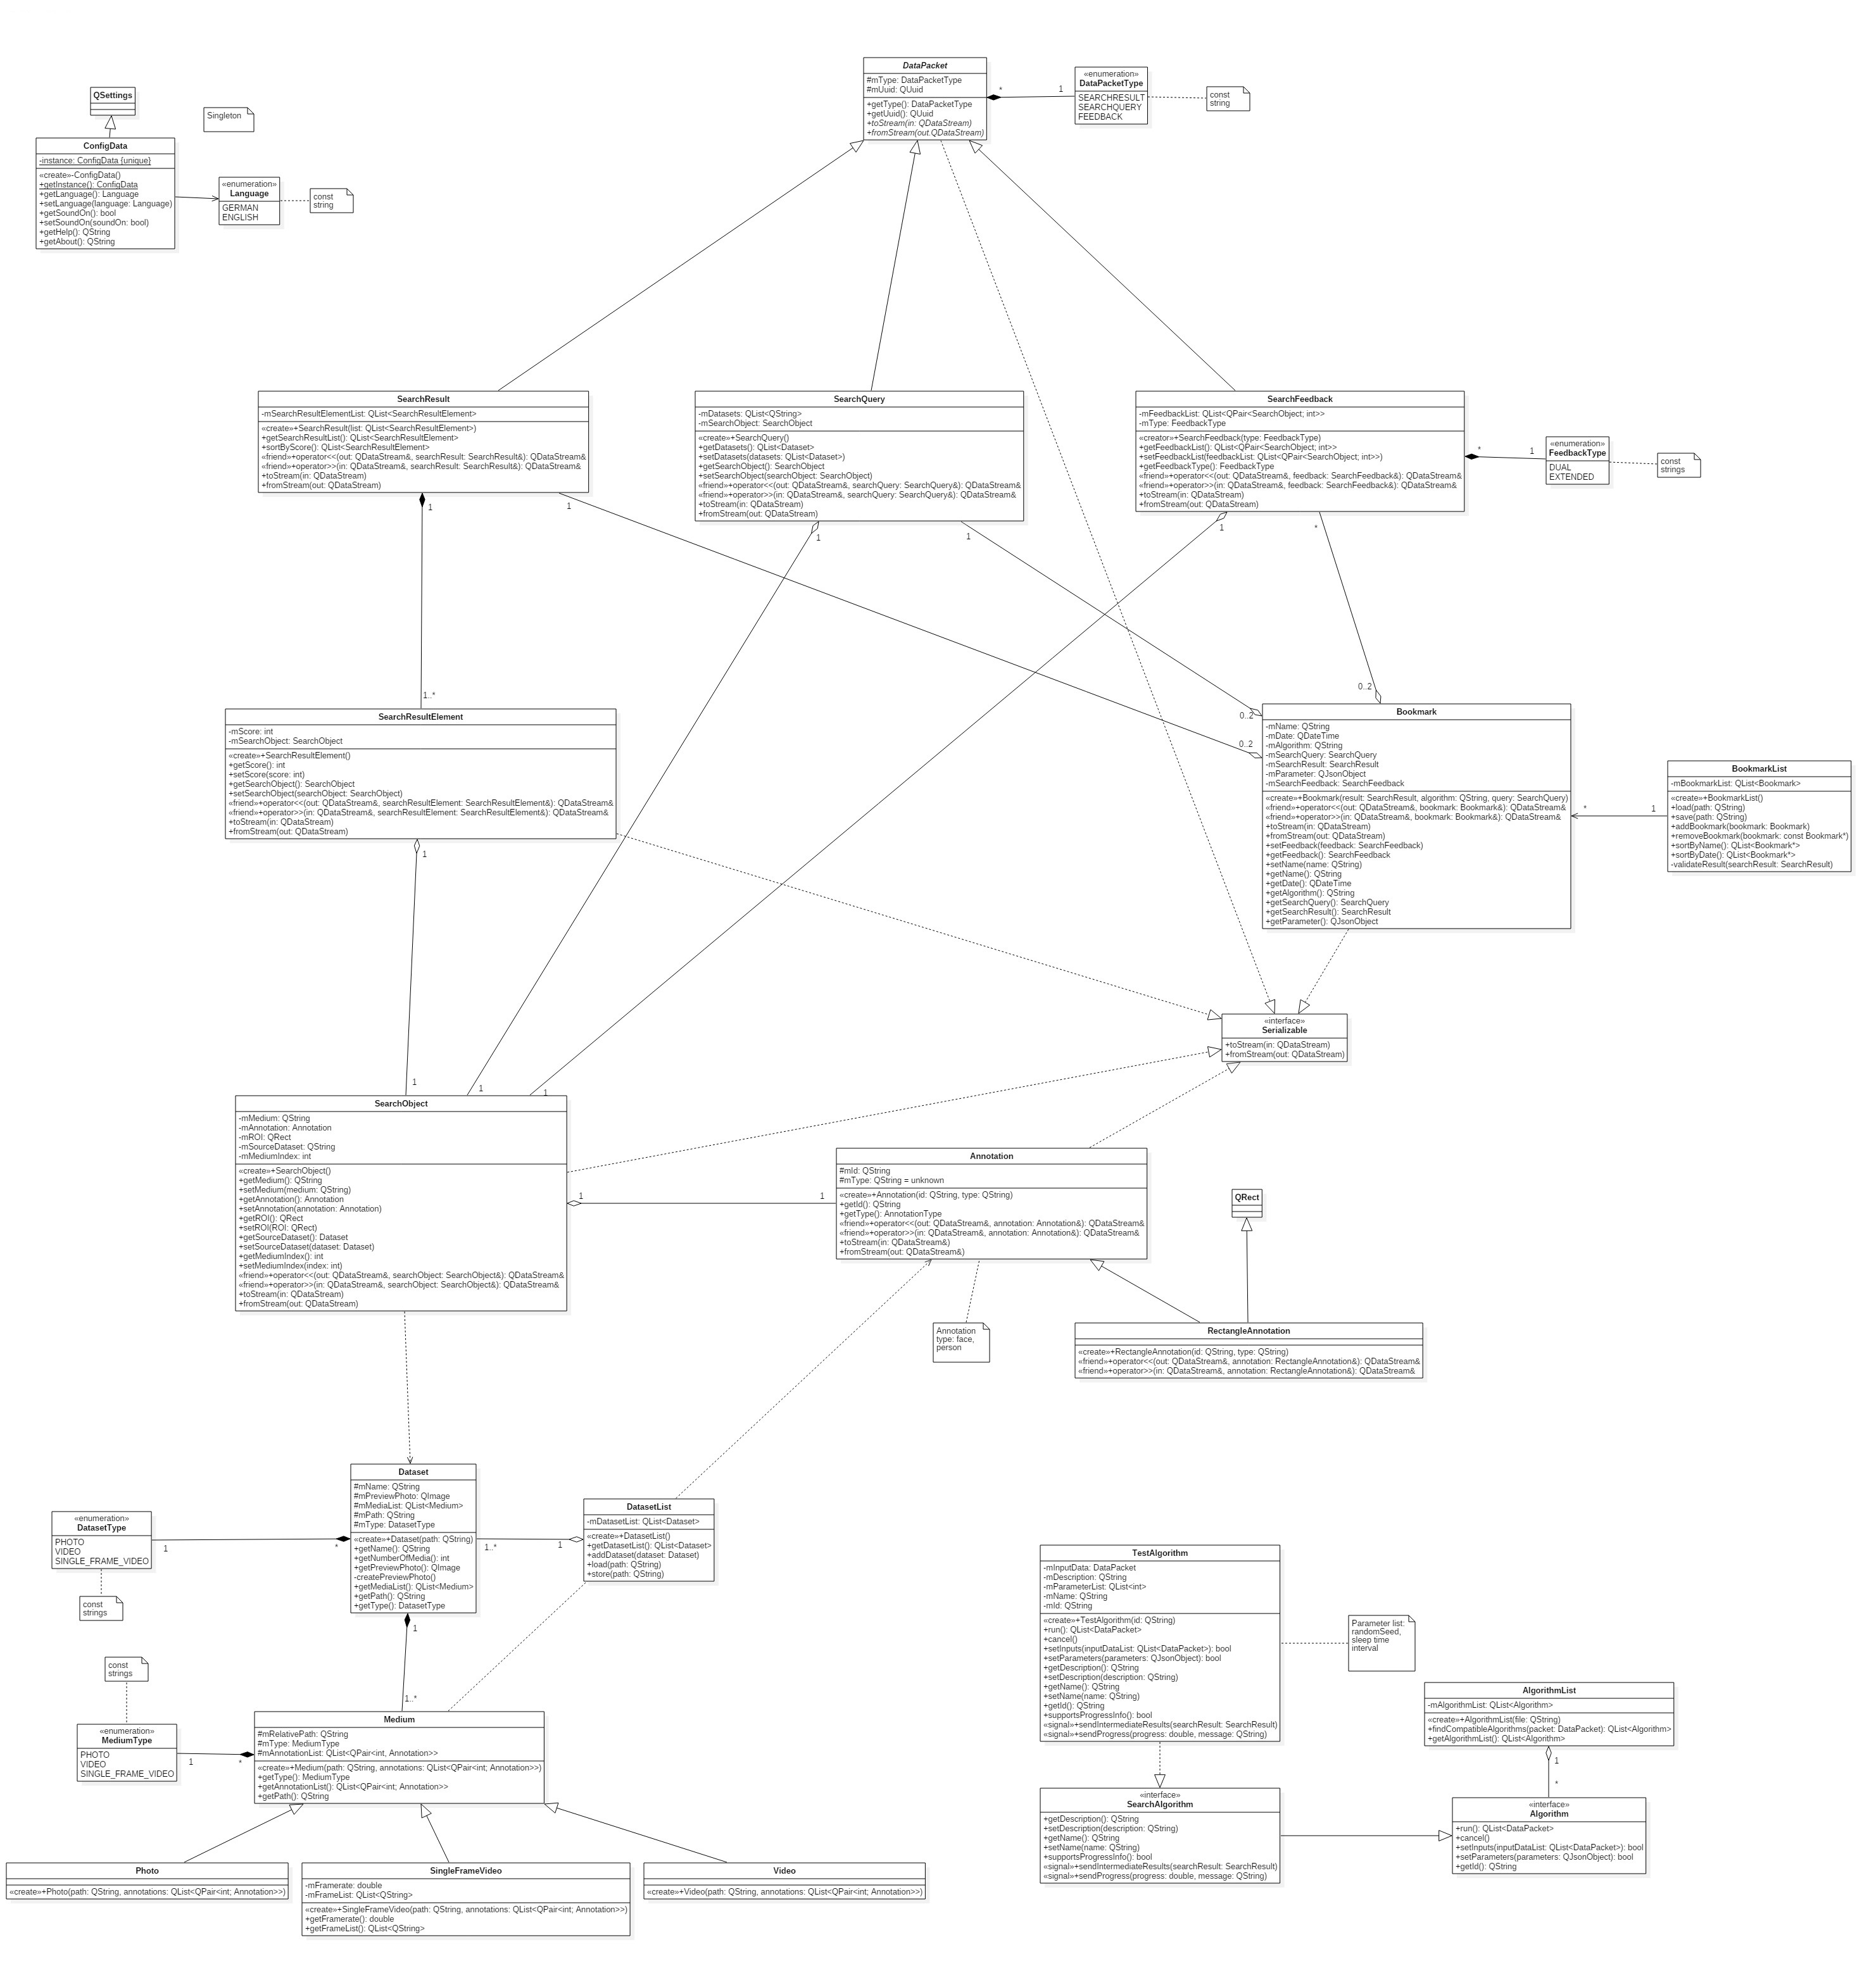
\includegraphics[width=1\linewidth]{img/Klassendiagramm/Model}
\caption{Model}
\label{fig:model}
\end{figure}


\subsection*{ConfigData}

Die Klasse ConfigData speichert die Benutzereinstellungen Sprache und Benachrichtigungston. Außerdem werden die Hilfe- und Aboutdateien gelesen.

\begin{figure}[H]
\centering
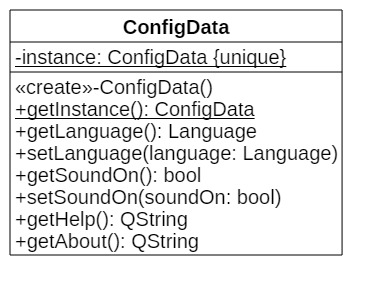
\includegraphics[scale=0.5]{img/Klassendiagramm/Klassen/Model/ConfigData}
\label{fig:configData}
\end{figure}

Attribute
\begin{itemize}
\item\textit{private ConfigData instance} Die einzige Instanz von ConfigData. 
\end{itemize}

Methoden
\begin{itemize}
\item \textit{private ConfigData()} Erzeugt ein neues ConfigData Objekt.
\item \textit{public static ConfigData getInstance()} Liefert die ConfigData Instanz zurück. Dies stellt sicher, dass nur eine Instanz von ConfigData existiert.
\item \textit{public Language getLanguage()} Lädt die vom Benutzer gewählte Sprache.
\item \textit{public void setLanguage(Language language)} Speichert die vom Benutzer gewählte Sprache.
\item \textit{public bool getSoundOn()} Lädt die vom Benutzer gewählte Toneinstellung.
\item \textit{public void setSoundOn(bool soundOn)} Speichert die vom Benutzer gewählte Toneinstellung.
\item \textit{public QString getHelp()} Lädt die Hilfedatei und gibt deren Inhalt zurück.
\item \textit{public QString getAbout()} Lädt die Aboutdatei und gibt deren Inhalt zurück.
\end{itemize}

\subsection*{<<enumeration>> Language}
Language repräsentiert die verfügbaren Sprachen: Deutsch und Englisch.

\begin{figure}[H]
\centering
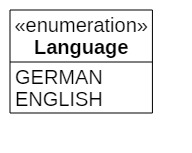
\includegraphics[scale=0.5]{img/Klassendiagramm/Klassen/Model/Language}
\label{fig:language}
\end{figure}

\subsection*{\gls{Annotation} : public Serializable}
Eine \gls{Annotation} ist ein in den Datensätzen vordefinierter Bereich eines Bildes oder Videos, der den Typ Face oder Person haben kann.

\begin{figure}[H]
\centering
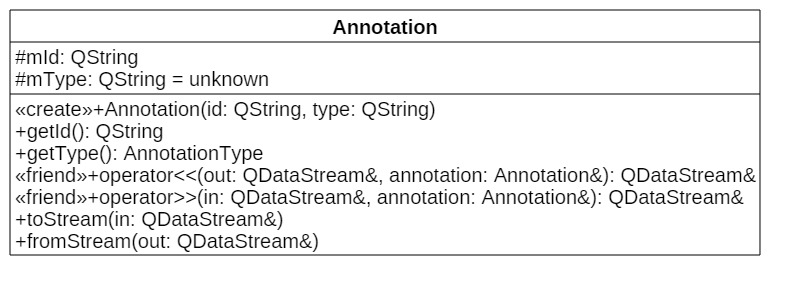
\includegraphics[scale=0.5]{img/Klassendiagramm/Klassen/Model/Annotation}
\label{fig:annotation}
\end{figure}

Attribute
\begin{itemize}
\item\textit{protected QString mId} Diese Id identifiziert diese \gls{Annotation} in einem  Medium.
\item\textit{protected QString mType} Beschreibt den Typ dieser \gls{Annotation}.
\end{itemize}

Methoden
\begin{itemize}
\item \textit{public Annotation(QString Id, QString type)} Gibt eine Instanz dieser Klasse zurück. Die übergebene Id identifiziert die \gls{Annotation} in einem Medium.
\item \textit{public QString getId()} Gibt die Id der \gls{Annotation} zurück.
\item \textit{public AnnotationType getType()} Gibt den Typ der \gls{Annotation} zurück.
\item \textit{public friend QDataStream\& operator<<(QDataStream\& out, Annotation\& annotation)} Speichert die \gls{Annotation} in einer Datei.
\item \textit{public friend QDataStream\& operator>>(QDataStream\& in, Annotation\& annotation)} Lädt die \gls{Annotation} aus einer Datei.
\item \textit{public void toStream(QDataStream in)} Speichert die \gls{Annotation}, durch den Aufruf von operator<<, in einer Datei.
\item \textit{public void fromStream(QDataStream out)} Lädt die \gls{Annotation}, durch den Aufruf von operator>>, aus einer Datei.
\end{itemize}

\subsection*{RectangleAnnotation : public Annotation, public QRect}
Eine rechteckige \gls{Annotation}.

\begin{figure}[H]
\centering
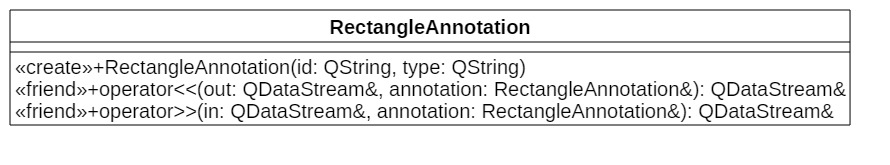
\includegraphics[scale=0.5]{img/Klassendiagramm/Klassen/Model/RectangleAnnotation}
\label{fig:rectangleAnnotation}
\end{figure}

Methoden
\begin{itemize}
\item \textit{public RectangleAnnotation(QString id, QString type)} Erzeugt ein Objekt von RectangleAnnotation. Die übergebene Id identifiziert die \gls{Annotation} in einem Medium.
\item \textit{public friend QDataStream\& operator<<(QDataStream\& out, RectangleAnnotation\& annotation)} Speichert die RectangleAnnotation in einer Datei.
\item \textit{public friend QDataStream\& operator>>(QDataStream\& in, RectangleAnnotation\& annotation)} Lädt die RectangleAnnotation aus einer Datei.
\end{itemize}

\subsection*{<<abstract>> DataPacket : public Serializable}
Ein DataPacket ist eine Eingabe für den \glslink{Suchalgorithmus}{Algorithmus}.

\begin{figure}[H]
\centering
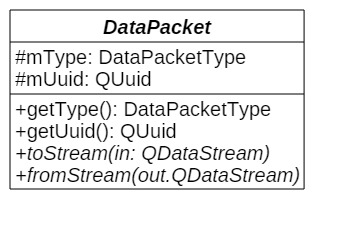
\includegraphics[scale=0.5]{img/Klassendiagramm/Klassen/Model/DataPacket}
\label{fig:dataPacket}
\end{figure}

Attribute
\begin{itemize}
\item\textit{protected DataPacketType mType} Beschreibt den Typ dieses DataPackets.
\item\textit{protected QUuid mUuid} Identifiziert dieses DataPacket eindeutig. 
\end{itemize}

Methoden
\begin{itemize}
\item \textit{public DataPacketType getType()} Gibt den Typ des DataPackets zurück, abhängig von der Kindklasse.
\item\textit{public QUuid getUuid} Gibt die eindeutige Id dieses DataPackets zurück.
\item \textit{public abstract void toStream(QDataStream in)} Speichert das DataPacket, durch den Aufruf von operator<<, in einer Datei.
\item \textit{public abstract void fromStream(QDataStream out)} Lädt das DataPacket, durch den Aufruf von operator>>, in einer Datei.
\end{itemize}

\pagebreak

\subsection*{<<enumeration>> DataPacketType}
DataPacketType enthält die Typen von DataPackets, also die vorhandenen Kindklassen.

\begin{figure}[H]
\centering
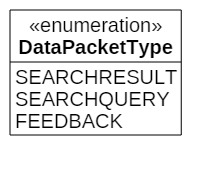
\includegraphics[scale=0.5]{img/Klassendiagramm/Klassen/Model/DataPacketType}
\label{fig:dataPacketType}
\end{figure}

\subsection*{SearchQuery : public DataPacket}
Eine SearchQuery ist eine Suchanfrage an den \glslink{Suchalgorithmus}{Algorithmus}.

\begin{figure}[H]
\centering
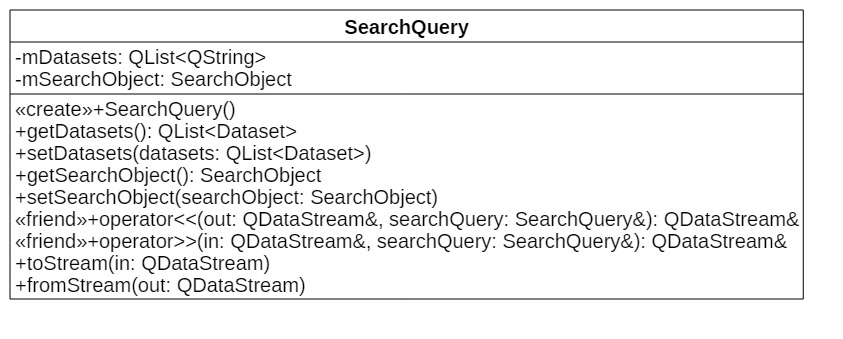
\includegraphics[scale=0.5]{img/Klassendiagramm/Klassen/Model/SearchQuery}
\label{fig:searchQuery}
\end{figure}

Attribute
\begin{itemize}
\item\textit{private QList<QString> mDatasets} Beschreibt den Suchraum der Suchanfrage.
\item\textit{private SearchObject mSearchObject} Das zu dieser Suchanfrage gehörende SearchObject.
\end{itemize}

Methoden
\begin{itemize}
\item \textit{public SearchQuery()} Erzeugt ein SearchQuery-Objekt.
\item \textit{public QList<Dataset> getDatasets()} Gibt den Suchraum, in Form von einer Datensatzliste, zurück.
\item \textit{public void setDatasets(QList<Dataset> datasets)} Setzt den Suchraum für die Suchanfrage.
\item \textit{public SearchObject getSearchObject()} Gibt das SearchObject für diese Anfrage zurück.
\item \textit{public void setSearchObject(SearchObject searchObject)} Setzt das SearchObject für diese Anfrage.
\item \textit{public friend QDataStream\& operator<<(QDataStream\& out, SearchQuery\& searchQuery)} Speichert die SearchQuery in einer Datei.
\item \textit{public friend QDataStream\& operator>>(QDataStream\& in, SearchQuery\& searchQuery)} Lädt die SearchQuery aus einer Datei.
\item \textit{public void toStream(QDataStream in)} Speichert die SearchQuery, durch den Aufruf von operator<<, in einer Datei.
\item \textit{public void fromStream(QDataStream out)} Lädt die SearchQuery, durch den Aufruf von operator>>, aus einer Datei.
\end{itemize}

\subsection*{SearchResult : public DataPacket}
Ein SearchResult ist die Ausgabe eines \glslink{Suchalgorithmus}{Algorithmus}. Allerdings kann es auch eine Eingabe sein, wenn ein \glslink{Suchalgorithmus}{Algorithmus} auf einem bestehenden Suchergebnis weiterarbeitet.

\begin{figure}[H]
\centering
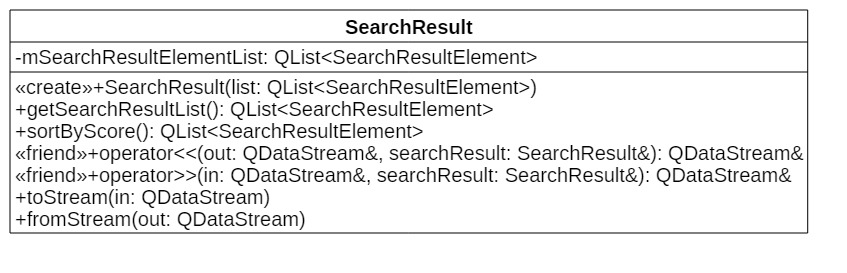
\includegraphics[scale=0.5]{img/Klassendiagramm/Klassen/Model/SearchResult}
\label{fig:searchResult}
\end{figure}

Attribute
\begin{itemize}
\item\textit{private QList<SearchResultElement> mSearchResultElementList} Die Liste der zu diesem SearchResult gehörenden SearchResultElements.
\end{itemize}

Methoden
\begin{itemize}
\item \textit{public SearchResult(QList<SearchResultElement> list)} Erzeugt ein neues SearchResult, das eine Liste von SearchResultElements enthält.
\item \textit{public QList<SearchResultElement> getSearchResultList()} Gibt die Liste der SearchResultElements zurück.
\item \textit{public void sortByScore()} Sortiert die Ergebnisliste nach dem Score.
\item \textit{public friend QDataStream\& operator<<(QDataStream\& out, SearchResult\& searchResult)} Speichert das SearchResult in einer Datei.
\item \textit{public friend QDataStream\& operator>>(QDataStream\& in, SearchResult\& searchResult)} Lädt das SearchResult aus einer Datei.
\item \textit{public void toStream(QDataStream in)} Speichert das SearchResult, durch den Aufruf von operator<<, in einer Datei.
\item \textit{public void fromStream(QDataStream out)} Lädt das SearchResult, durch den Aufruf von operator>>, aus einer Datei.
\end{itemize}

\subsubsection*{SearchResultElement : public Serializable}
Ein SearchResultElement ist ein Element von SearchResult. Abgesehen von einem SearchObject enthält es einen Score für dieses, der durch den \glslink{Suchalgorithmus}{Algorithmus} bestimmt und gesetzt wurde.

\begin{figure}[H]
\centering
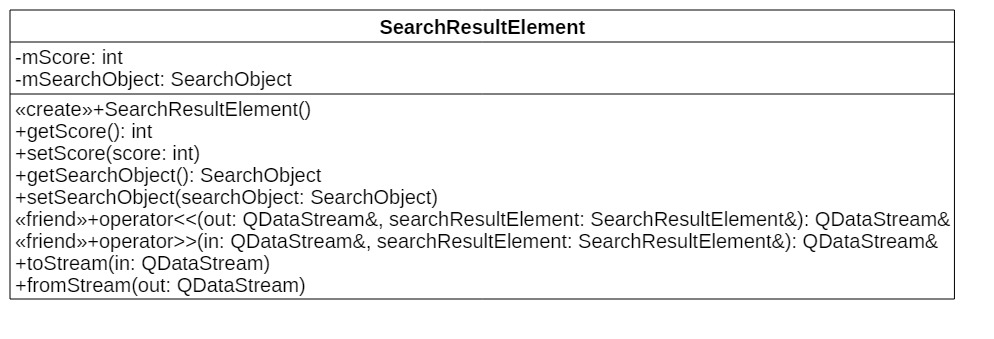
\includegraphics[width=\linewidth]{img/Klassendiagramm/Klassen/Model/SearchResultElement}
\label{fig:searchResultElement}
\end{figure}

Attribute
\begin{itemize}
\item\textit{private int mScore} Vom \gls{Suchalgorithmus} zugewiesene Zahl, die die Ähnlichkeit dieses SearchResultElements mit der Suchanfrage beschreibt. 
\item\textit{private SearchObject mSearchObject} Das zu diesem SearchResultElement gehörende SearchObject.
\end{itemize}

Methoden
\begin{itemize}
\item \textit{public SearchResultElement()} Erzeugt ein SearchResultElement.
\item \textit{public int getScore()} Gibt den Score für dieses Element zurück.
\item \textit{public void setScore(int score)} Setzt den Score für dieses Element.
\item \textit{public SearchObject getSearchObject()} Gibt das SearchObject zurück.
\item \textit{public void setSearchObject(SearchObject searchObject)} Setzt das übergebene SearchObject für das Element.
\item \textit{public friend QDataStream\& operator<<(QDataStream\& out, SearchResultElement\& searchResultElement)} Speichert das SearchResultElement in einer Datei.
\item \textit{public friend QDataStream\& operator>>(QDataStream\& in, SearchResultElement\& searchResultElement)} Lädt das SearchResultElement aus einer Datei.
\item \textit{public void toStream(QDataStream in)} Speichert das SearchResultElement, durch den Aufruf von operator<<, in einer Datei.
\item \textit{public void fromStream(QDataStream out)} Lädt das SearchResultElement, durch den Aufruf von operator>>, aus einer Datei.
\end{itemize}

\subsection*{SearchObject : public Serializable}
Das SearchObject repräsentiert eine \gls{Annotation} oder ein Rechteck in einem Bild oder Frame eines Videos aus einem Datensatz.

\begin{figure}[H]
\centering
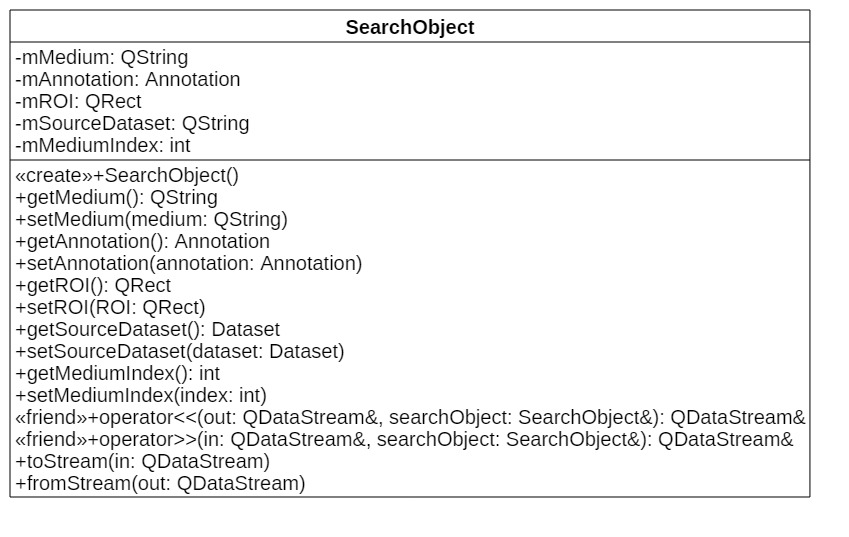
\includegraphics[scale=0.5]{img/Klassendiagramm/Klassen/Model/SearchObject}
\label{fig:searchObject}
\end{figure}

Attribute
\begin{itemize}
\item\textit{private QString mMedium} Der Pfad des zugehörigen Mediums.
\item\textit{private Annotation mAnnotation} Die ausgewählte \gls{Annotation}.
\item\textit{private QRect mROI} Die \glslink{ROI}{\enquote{region of interest}} im zugehörigen Medium.
\item\textit{private QString mSourceDataset} Der Pfad des Datensatzes, in dem sich das Medium befindet.
\item\textit{private int mMediumIndex} Beschreibt die Framenummer des Mediums in einem Video.
\end{itemize}

Methoden
\begin{itemize}
\item \textit{public SearchObject} Erzeugt ein SearchObject.
\item \textit{public QString getMedium()} Gibt den Dateipfad des Mediums zurück.
\item \textit{public void setMedium(QString medium)} Setzt das Medium auf den gegebenen Dateipfad, relativ zum SourceDataset.
\item \textit{public Annotation getAnnotation()} Gibt die \gls{Annotation} im Medium zurück.
\item \textit{public void setAnnotation(Annotation annotation)} Setzt eine \gls{Annotation} eines Mediums für das SearchObject.
\item \textit{public QRect getROI()} Gibt ein QRect zurück, das die \glslink{ROI}{\enquote{region of interest}} im Medium repräsentiert.
\item \textit{public void setROI(QRect ROI)} Setzt ein QRect als \gls{ROI}.
\item \textit{public Dataset getSourceDataset} Gibt den Datensatz, in dem sich das Medium befindet, zurück.
\item \textit{public void setSourceDataset(Dataset dataset)} Setzt den Datensatz, in dem sich das Medium befindet.
\item \textit{public int getMediumIndex()} Gibt den Index eines Mediums, also den Frame in einem Video, zurück.
\item \textit{public void setMediumIndex(int index)} Setzt den MediumIndex.
\item \textit{public friend QDataStream\& operator<<(QDataStream\& out, SearchObject\& searchObject)} Speichert das SearchObject in einer Datei.
\item \textit{public friend QDataStream\& operator>>(QDataStream\& in, SearchObject\& searchObject)} Lädt das SearchObject aus einer Datei.
\item \textit{public void toStream(QDataStream in)} Speichert das SearchObject, durch den Aufruf von operator<<, in einer Datei.
\item \textit{public void fromStream(QDataStream out)} Lädt das SearchObject, durch den Aufruf von operator>>, aus einer Datei.
\end{itemize}

\subsection*{SearchFeedback : public DataPacket}
Das SearchFeedback gibt an, wie gut das vom \glslink{Suchalgorithmus}{Algorithmus} erzeugte Suchergebnis ist.

\begin{figure}[H]
\centering
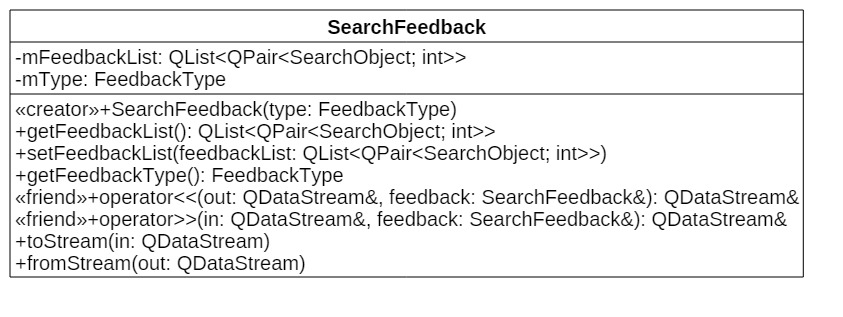
\includegraphics[scale=0.5]{img/Klassendiagramm/Klassen/Model/SearchFeedback}
\label{fig:searchFeedback}
\end{figure}

Attribute
\begin{itemize}
\item\textit{private QList<QPair<SearchObject, int>}> Der Integer-Wert beschreibt das zum SearchObject gehörende Feedback.
\item\textit{private FeedbackType mType} Der Typ des Feedbacks, entweder dual oder extended.
\end{itemize}

Methoden
\begin{itemize}
\item \textit{public SearchFeedback(FeedbackType type)} Erzeugt ein neues SearchFeedback Objekt. Der Typ kann entweder dual oder extended sein.
\item \textit{public QList<QPair<SearchObject, int>}\textit{>  getFeedbackList()} Gibt die FeedbackList  zurück.
\item \textit{public void setFeedbackList(QList<QPair<SearchObject, int>}\textit{> feedbackList)} Setzt die FeedbackList auf die übergebene Liste.
\item \textit{public FeedbackType getFeedbackType()} Gibt den Feedback-Typ zurück.
\item \textit{public friend QDataStream\& operator<<(QDataStream\& out, Feedback\& feedback)} Speichert das Feedback in einer Datei.
\item \textit{public friend QDataStream\& operator>>(QDataStream\& in, Feedback\& feedback)} Lädt das Feedback aus einer Datei.
\item \textit{public void toStream(QDataStream in)} Speichert das Feedback, durch den Aufruf von operator<<, in einer Datei.
\item \textit{public void fromStream(QDataStream out)} Lädt das Feedback, durch den Aufruf von operator>>, aus einer Datei.
\end{itemize} 

\subsubsection*{<<enumeration>> FeedbackType}
Der FeedbackType kann dual (positiv, negativ, neutral) oder extended (Werte von 1 bis 10) sein.

\begin{figure}[H]
\centering
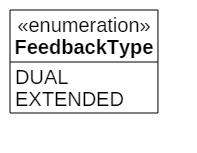
\includegraphics[scale=0.5]{img/Klassendiagramm/Klassen/Model/FeedbackType}
\label{fig:feedbackType}
\end{figure}

\subsection*{<<interface>> Serializable}
Das Interface Serializable dient dazu, die implementierenden Klassen serialisierbar zu machen.

\begin{figure}[H]
\centering
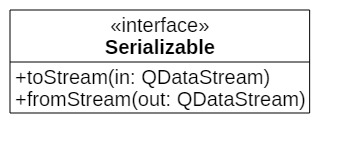
\includegraphics[scale=0.5]{img/Klassendiagramm/Klassen/Model/Serializable}
\label{fig:serializable}
\end{figure}

Methoden
\begin{itemize}
\item \textit{public void toStream(QDataStream in)} Speichert das serialisierbare Objekt in einer Datei.
\item \textit{public void fromStream(QDataStream out)} Lädt das serialisierbare Objekt aus einer Datei.
\end{itemize}

\subsection*{Bookmark : public Serializable}
Ein Bookmark speichert ein Suchergebnis, eine Suchanfrage und das Feedback, sodass ein früherer Suchvorgang wiederhergestellt werden kann.

\begin{figure}[H]
\centering
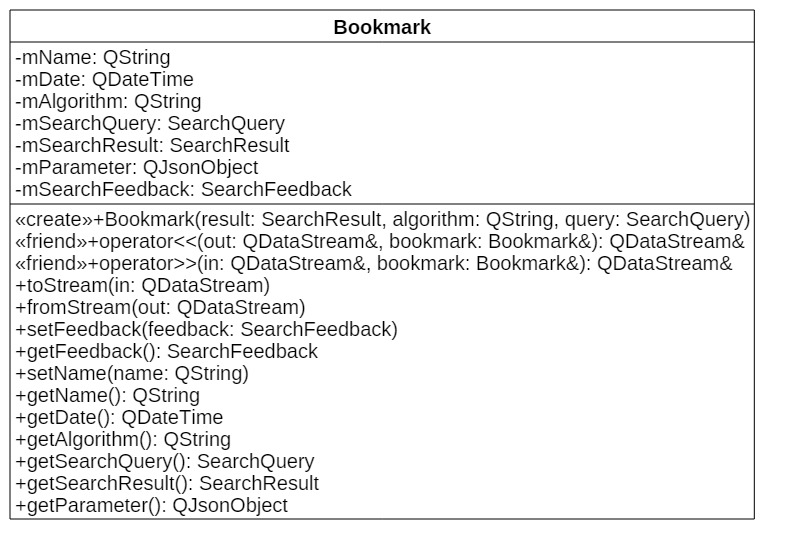
\includegraphics[scale=0.5]{img/Klassendiagramm/Klassen/Model/Bookmark}
\label{fig:bookmark}
\end{figure}

Attribute
\begin{itemize}
\item\textit{private QString mName} Der Name dieses Bookmarks.
\item\textit{private QDateTime mDate} Die Zeit, zu der das Bookmark gespeichet wurde.
\item\textit{private QString mAlgorithm} Der Name des \glslink{Suchalgorithmus}{Algorithmus}, der für diese Suche eingesetzt wurde.
\item\textit{private SearchQuery mSearchQuery} Die Suchanfrage dieser Suche.
\item\textit{private SearchResult mSearchResult} Das Suchergebnis dieser Suche.
\item\textit{private QJsonObject mParameter} Die für diese Suche gesetzten Parameter.
\item\textit{private SearchFeedback mSearchFeedback} Das vom Benutzer gesetzte Feedback.
\end{itemize}


Methoden
\begin{itemize}
\item \textit{public Bookmark(SearchResult result, QString algorithm, SearchQuery query)} Erzeugt ein neues Bookmark.
\item \textit{public friend QDataStream\& operator<<(QDataStream\& out, Bookmark\& bookmark)} Speichert das Bookmark in einer Datei.
\item \textit{public friend QDataStream\& operator>>(QDataStream\& in, Bookmark\& bookmark)} Lädt das Bookmark aus einer Datei.
\item \textit{public void toStream(QDataStream in)} Speichert das Bookmark, durch den Aufruf von operator<<, in einer Datei.
\item \textit{public void fromStream(QDataStream out)} Lädt das Bookmark, durch den Aufruf von operator>>, aus einer Datei.
\item\textit{public void setFeedback(SearchFeedback feedback)} Speichert das Feedback im Bookmark.
\item\textit{public SearchFeedback getFeedback()} Gibt das Feedback zurück.
\item\textit{public void setName(QString name)} Setzt den Namen des Bookmarks.
\item\textit{public QString getName()} Gibt den Namen des Bookmarks zurück.
\item\textit{public QDateTime getDate()} Gibt die Zeit, zu der das Bookmark erstellt wurde, zurück.
\item\textit{public QString getAlgorithm()} Gibt den Namen des verwendeten \glslink{Suchalgorithmus}{Algorithmus} zurück.
\item\textit{public SearchQuery getSearchQuery()} Gibt die Suchanfrage zurück.
\item\textit{public SearchResult getSearchResult()} Gibt das Suchergebnis zurück.
\item\textit{public QJsonObject getParameter()} Gibt die Parameter zurück.
\end{itemize}

\subsection*{BookmarkList}
Die BookmarkList hält eine Liste von Bookmarks und speichert die Bookmarks.

\begin{figure}[H]
\centering
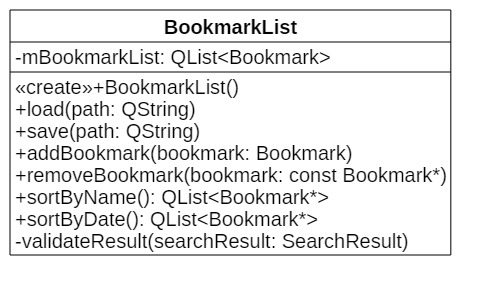
\includegraphics[scale=0.5]{img/Klassendiagramm/Klassen/Model/BookmarkList}
\label{fig:bookmarkList}
\end{figure}

Attribute
\begin{itemize}
\item\textit{private QList<Bookmark> mBookmarkList} Eine Liste von Bookmarks.
\end{itemize}

Methoden
\begin{itemize}
\item \textit{public BookmarkList()} Erzeugt eine BookmarkList.
\item \textit{public void load(QString path)} Lädt die Bookmarks aus der Datei.
\item \textit{public void save(QString path)} Speichert die Bookmark Liste in der Datei mit dem übergebenen Pfad.
\item \textit{public void addBookmark(Bookmark bookmark)} Fügt ein Bookmark in die Liste ein.
\item \textit{public void removeBookmark(const Bookmark* bookmark)} Entfernt das Bookmark aus der BookmarkList.
\item \textit{public QList<Bookmark*> sortByName()} Gibt die nach Namen sortierte Bookmarkliste zurück.
\item \textit{public QList<Bookmark*> sortByDate()} Gibt die nach Datum sortierte Bookmarkliste zurück.
\item \textit{private void validateResult(SearchResult searchResult)} Überprüft, ob das übergebene SearchResult gültig ist, also noch alle Datensätze und Medien vorhanden sind.
\end{itemize}

\subsection*{Dataset}
Ein Dataset hat einen Typ und enthält Medien von diesem Typ.

\begin{figure}[H]
\centering
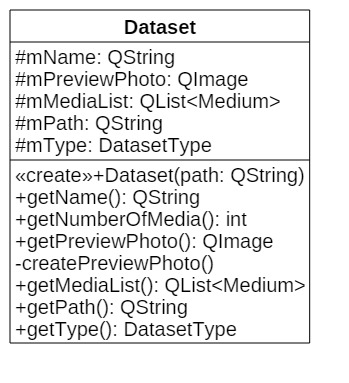
\includegraphics[scale=0.5]{img/Klassendiagramm/Klassen/Model/Dataset}
\label{fig:dataset}
\end{figure}

Attribute
\begin{itemize}
\item\textit{protected QString mName} Der Name des Ordners.
\item\textit{protected QImage mPreviewPhoto} Das Vorschaubild dieses Datensatzes.
\item\textit{protected QList<Medium> mMediaList} Die Liste der Medien in diesem Datensatz.
\item\textit{protected QString mPath} Der Pfad dieses Datensatzes.
\item\textit{protected DatasetType mType} Der Typ dieses Datensatzes.
\end{itemize}

Methoden
\begin{itemize}
\item \textit{public Dataset(QString path)} Erzeugt einen Datensatz mit dem übergebenen Ordnerpfad.
\item \textit{public QString getName()} Gibt den Namen des Datensatzes (des Ordners) zurück.
\item \textit{public int getNumberOfMedia()} Gibt die Anzahl der Medien in der MediaList zurück.
\item \textit{public QImage getPreviewPhoto()} Gibt das Vorschaubild des Datensatzes zurück.
\item \textit{private void createPreviewPhoto()} Erstellt ein Vorschaubild aus den Medien.
\item \textit{public QList<Medium> getMediaList()} Gibt die Liste aller Medien zurück.
\item \textit{public QString getPath()} Gibt den absoluten Pfad des Datensatzes zurück.
\item \textit{public DatasetType getType()} Gibt den Typ des Datensatzes (und damit auch der Medien) zurück.
\end{itemize}

\subsection*{DatasetList}
Eine DatasetList hält eine Liste von Datensätzen und speichert sie.

\begin{figure}[H]
\centering
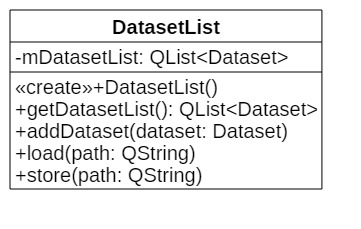
\includegraphics[scale=0.5]{img/Klassendiagramm/Klassen/Model/DatasetList}
\label{fig:datasetList}
\end{figure}

Attribute
\begin{itemize}
\item\textit{private QList<Dataset> mDatasetList} Die Liste von Datensätzen.
\end{itemize}

Methoden
\begin{itemize}
\item \textit{public DatasetList()} Erzeugt eine DatasetList.
\item \textit{public QList<Dataset> getDatasetList()} Gibt die Liste der Datensätze zurück.
\item \textit{public void addDataset(Dataset dataset)} Fügt den übergebenen Dataset der Liste hinzu.
\item \textit{public void load(QString path)} Lädt die Datensatzliste aus der Datei mit dem übergebenen Pfad.
\item \textit{public void store(QString path)} Speichert die Datensatzliste in der Datei mit dem übergebenen Pfad.
\end{itemize}

\subsection*{DatasetType}
Der Datensatztyp kann Photo, Video oder SingleFrameVideo sein.

\begin{figure}[H]
\centering
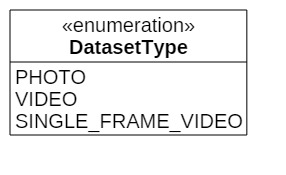
\includegraphics[scale=0.5]{img/Klassendiagramm/Klassen/Model/DatasetType}
\label{fig:datasetType}
\end{figure}

\subsection*{Medium}
Ein Medium wird durch einen Pfad charakterisiert. Außerdem hat ein Medium eine Liste von \glslink{Annotation}{Annotationen} und den zugehörigen Index. Der Index ist bei Photos 0, in Videos gibt er an, in welchem Frame sich die \gls{Annotation} befindet.

\begin{figure}[H]
\centering
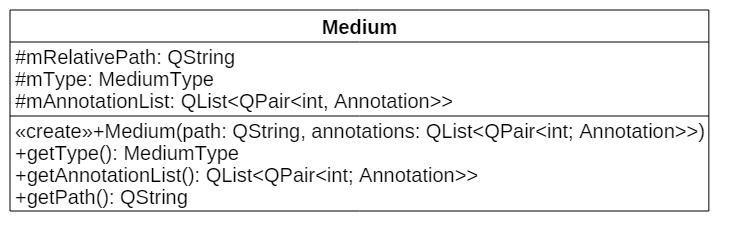
\includegraphics[scale=0.5]{img/Klassendiagramm/Klassen/Model/Medium}
\label{fig:medium}
\end{figure}

Attribute
\begin{itemize}
\item\textit{protected QString mRelativePath} Der Pfad zu diesem Medium.
\item\textit{protected MediumType mType} Der Typ dieses Mediums.
\item\textit{protected QList<QPair<int, Annotation>}\textit{> mAnnotationList} Die Liste von \glslink{Annotation}{Annotationen} für dieses Medium.
\end{itemize}

Methoden
\begin{itemize}
\item \textit{public Medium(QString path, QList<QPair<int, Annotation>}\textit{> annotations)} Erzeugt ein Medium, das den übergebenen Pfad und die \glslink{Annotation}{Annotationsliste} hat.
\item \textit{public MediumType getType()} Gibt den Typ des Mediums zurück.
\item \textit{public QList<QPair<int, Annotation>}> Gibt die Liste der \glslink{Annotation}{Annotationen} zurück.
\end{itemize}

\subsection*{<<enumeration>> MediumType}
Der MediumType gibt den Typ des Mediums an: Photo, Video oder SingleFrameVideo.

\begin{figure}[H]
\centering
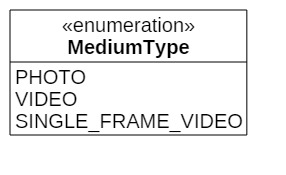
\includegraphics[scale=0.5]{img/Klassendiagramm/Klassen/Model/MediumType}
\label{fig:mediumType}
\end{figure}

\subsection*{Photo : public Medium}
Ein Photo ist ein Bild, in dem \glslink{Annotation}{Annotationen} sein können.

\begin{figure}[H]
\centering
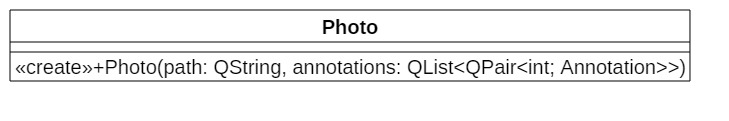
\includegraphics[scale=0.5]{img/Klassendiagramm/Klassen/Model/Photo}
\label{fig:photo}
\end{figure}

Methoden
\begin{itemize}
\item \textit{public Photo(QString path)} Erzeugt ein Photo mit dem übergebenen Pfad.
\end{itemize}

\subsection*{SingleFrameVideo : public Medium}
Ein SingleFrameVideo ist ein Video aus Einzelbildern.

\begin{figure}[H]
\centering
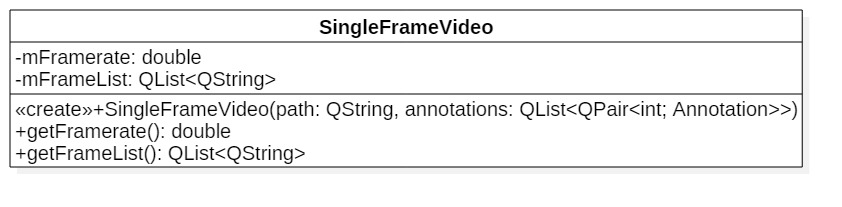
\includegraphics[scale=0.5]{img/Klassendiagramm/Klassen/Model/SingleFrameVideo}
\label{fig:singleFrameVideo}
\end{figure}

Attribute
\begin{itemize}
\item\textit{private double mFramerate} Die Framerate dieses Videos.
\item\textit{private QList<QString> mFrameList} Die Liste von Frames dieses Videos.
\end{itemize}

Methoden
\begin{itemize}
\item \textit{public SingleFrameVideo(QString path)} Erzeugt ein SingleFrameVideo.
\item \textit{public double getFramerate()} Gibt die Framerate des Videos zurück.
\item \textit{public QList<QString> getFrameList()} Gibt die Liste der Frames zurück.
\end{itemize}

\subsection*{Video : public Medium}
Ein Video aus einer Videodatei.

\begin{figure}[H]
\centering
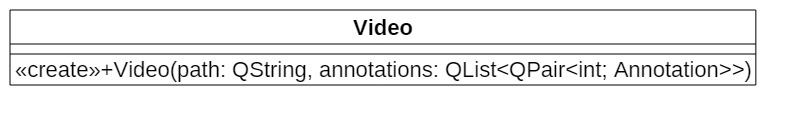
\includegraphics[scale=0.5]{img/Klassendiagramm/Klassen/Model/Video}
\label{fig:video}
\end{figure}

Methoden
\begin{itemize}
\item \textit{public Video(QString path)} Erzeugt ein Video aus dem übergebenen Pfad.
\end{itemize}

\subsection*{<<interface>> \glslink{Suchalgorithmus}{Algorithm}}
Die \glslink{Suchalgorithmus}{Algorithmen}, die von CoBaB ausgeführt werden sollen, müssen mindestens diese Schnittstelle implementieren.

\begin{figure}[H]
\centering
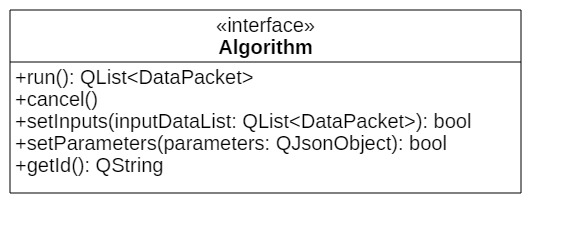
\includegraphics[scale=0.5]{img/Klassendiagramm/Klassen/Model/Algorithm}
\label{fig:algorithm}
\end{figure}

Methoden
\begin{itemize}
\item\textit{public QList<DataPacket> run()} Startet den \glslink{Suchalgorithmus}{Algorithmus}. Die Liste von DataPackets sind die Ergebnisse des \glslink{Suchalgorithmus}{Algorithmus}.
\item\textit{public void cancel()} Bricht die Ausführung des \glslink{Suchalgorithmus}{Algorithmus} ab.
\item\textit{public bool setInputs(QList<DataPacket> inputDataList)} Übergibt die benötigten Daten an den \glslink{Suchalgorithmus}{Algorithmus}. Der \glslink{Suchalgorithmus}{Algorithmus} gibt zurück, ob diese Liste seinen Eingabeparametern entspricht und es somit möglich ist, ihn zu starten.
\item\textit{public bool setParameters(QJsonObject parameters)} Übergibt die vom Benutzer festgelegten Parameterwerte an den \glslink{Suchalgorithmus}{Algorithmus}. Der \glslink{Suchalgorithmus}{Algorithmus} gibt zurück, ob diese Parameterdatei für ihn geeignet ist.
\item\textit{public QString getId()} Gibt eine für diesen \glslink{Suchalgorithmus}{Algorithmus} eindeutige Identifikation zurück.
\end{itemize}

\pagebreak

\subsection*{<<interface>> \glslink{Suchalgorithmus}{SearchAlgorithm} : public Algorithm}
Die Implementierung dieser Schnittstelle ermöglicht CoBaB, genauere Angaben über den \glslink{Suchalgorithmus}{Algorithmus} anzuzeigen.

\begin{figure}[H]
\centering
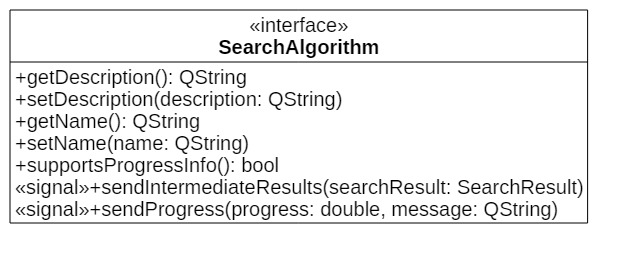
\includegraphics[scale=0.5]{img/Klassendiagramm/Klassen/Model/SearchAlgorithm}
\label{fig:searchAlgorithm}
\end{figure}

Methoden
\begin{itemize}
\item\textit{public QString getDescription()} Gibt eine Beschreibung des \glslink{Suchalgorithmus}{Algorithmus} zurück.
\item\textit{public void setDescription(QString description)} Setzt die Beschreibung des \glslink{Suchalgorithmus}{Algorithmus}.
\item\textit{public QString getName()} Gibt den Namen des \glslink{Suchalgorithmus}{Algorithmus} zurück.
\item\textit{public void setName(QString name)} Setzt den Namen des \glslink{Suchalgorithmus}{Algorithmus} auf name.
\item\textit{public bool supportsProgressInfo()} Gibt zurück, ob der \glslink{Suchalgorithmus}{Algorithmus} Fortschrittsinformationen senden kann.
\item\textit{public signal sendIntermediateResults(SearchResult searchResult)} Ist ein Signal, dass vom \glslink{Suchalgorithmus}{Algorithmus} gesendet wird, wenn Zwischenergebnisse verfügbar sind.
\item\textit{public signal sendProgress(double progress, QString message)} Ist ein Signal, das den Fortschritt des \glslink{Suchalgorithmus}{Algorithmus} sendet.
\end{itemize}

\pagebreak

\subsection*{TestAlgorithm : public SearchAlgorithm}
Dieser \gls{Suchalgorithmus} wird zu Testzwecken implementiert. Er generiert ein zufälliges SearchResult.

\begin{figure}[H]
\centering
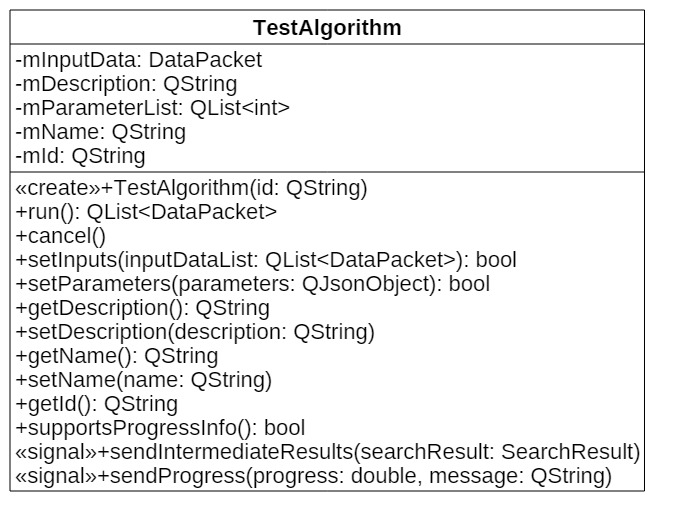
\includegraphics[scale=0.5]{img/Klassendiagramm/Klassen/Model/TestAlgorithm}
\label{fig:testAlgorithm}
\end{figure}

Attribute
\begin{itemize}
\item\textit{private DataPacket mInputData} Die Eingabedaten für den \glslink{Suchalgorithmus}{Algorithmus}.
\item\textit{private QString mDescription} Die Beschreibung für den \glslink{Suchalgorithmus}{Algorithmus}.
\item\textit{private QList<int> mParameterList} Mögliche Einträge für die Parameterliste: randomSeed, sleep time interval.
\item\textit{private QString mName} Der Name des \glslink{Suchalgorithmus}{Algorithmus}.
\item\textit{private QString mId} Die Id des \glslink{Suchalgorithmus}{Algorithmus}.
\end{itemize}

Methoden
\begin{itemize}
\item\textit{public TestAlgorithm(QString id)} Erstellt einen neuen \glslink{Suchalgorithmus}{Test-Algorithmus}.
\item\textit{public QList<DataPacket> run()} Startet den \glslink{Suchalgorithmus}{Algorithmus}. Die Liste von DataPackets sind die Ergebnisse des \glslink{Suchalgorithmus}{Algorithmus}.
\item\textit{public void cancel()} Bricht die Ausführung des \glslink{Suchalgorithmus}{Algorithmus} ab.
\item\textit{public bool setInputs(QList<DataPacket> inputDataList)} Übergibt die benötigten Daten an den \glslink{Suchalgorithmus}{Algorithmus}. Der \glslink{Suchalgorithmus}{Algorithmus} gibt zurück, ob diese Liste seinen Eingabeparametern entspricht und es somit möglich ist, ihn zu starten.
\item\textit{public bool setParameters(QJsonObject parameters)} Übergibt die vom Benutzer festgelegten Parameterwerte an den Algorithmus. Der Algorithmus gibt zurück, ob diese Parameterdatei für ihn geeignet ist.
\item\textit{public QString getId()} Gibt eine für diesen \glslink{Suchalgorithmus}{Algorithmus} eindeutige Identifikation zurück.
\item\textit{public QString getDescription()} Gibt eine Beschreibung des \glslink{Suchalgorithmus}{Algorithmus} zurück.
\item\textit{public void setDescription(QString description)} Setzt die Beschreibung für den \glslink{Suchalgorithmus}{Algorithmus}.
\item\textit{public QString getName()} Gibt den Namen des \glslink{Suchalgorithmus}{Algorithmus} zurück.
\item\textit{public void setName(QString name)} Setzt den Namen des \glslink{Suchalgorithmus}{Algorithmus} auf name.
\item\textit{public QString getId()} Gibt die Id des \glslink{Suchalgorithmus}{Algorithmus} zurück.
\item\textit{public bool supportsProgressInfo()} Gibt zurück, ob der \glslink{Suchalgorithmus}{Algorithmus} Fortschrittsinformationen senden kann.
\item\textit{public signal sendIntermediateResults(SearchResult searchResult)} Ist ein Signal, dass vom \glslink{Suchalgorithmus}{Algorithmus} gesendet wird, wenn Zwischenergebnisse verfügbar sind.
\item\textit{public signal sendProgress(double progress, QString message)} Ist ein Signal, das den Fortschritt des \glslink{Suchalgorithmus}{Algorithmus} sendet.
\end{itemize}

\pagebreak

\subsection*{AlgorithmList}
Diese Liste verwaltet verfügbare \glslink{Suchalgorithmus}{Algorithmen}.

\begin{figure}[H]
\centering
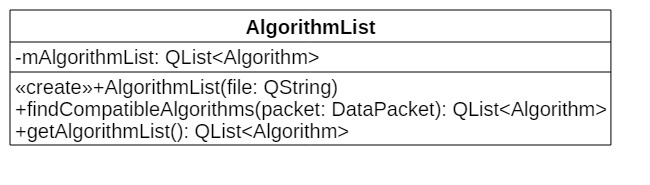
\includegraphics[scale=0.5]{img/Klassendiagramm/Klassen/Model/AlgorithmList}
\label{fig:algorithmList}
\end{figure}

Attribute
\begin{itemize}
\item\textit{private QList<Algorithm> mAlgorithmList} Die Liste der verfügbaren \glslink{Suchalgorithmus}{Algorithmen}.
\end{itemize}

Methoden
\begin{itemize}
\item\textit{public AlgorithmList(QString file)} Erzeugt eine Liste der verfügbaren \glslink{Suchalgorithmus}{Algorithmen}.
\item\textit{public QList<Algorithm> findCompatibleAlgorithms(DataPacket packet)} Gibt das DataPacket als Eingabe an alle \glslink{Suchalgorithmus}{Algorithmen} und gibt die Liste der \glslink{Suchalgorithmus}{Algorithmen} zurück, die diese Eingabe akzeptiert haben.
\item\textit{public QList<Algorithm> getAlgorithmList()} Gibt die Liste der verfügbaren \glslink{Suchalgorithmus}{Algorithmen} zurück.
\end{itemize}

\pagebreak

\subsection{View}

Dieses Diagramm zeigt alle Klassen des Views. Die zugehörigen Attribute und Methoden werden im Folgenden beschrieben.

\begin{figure}[H]
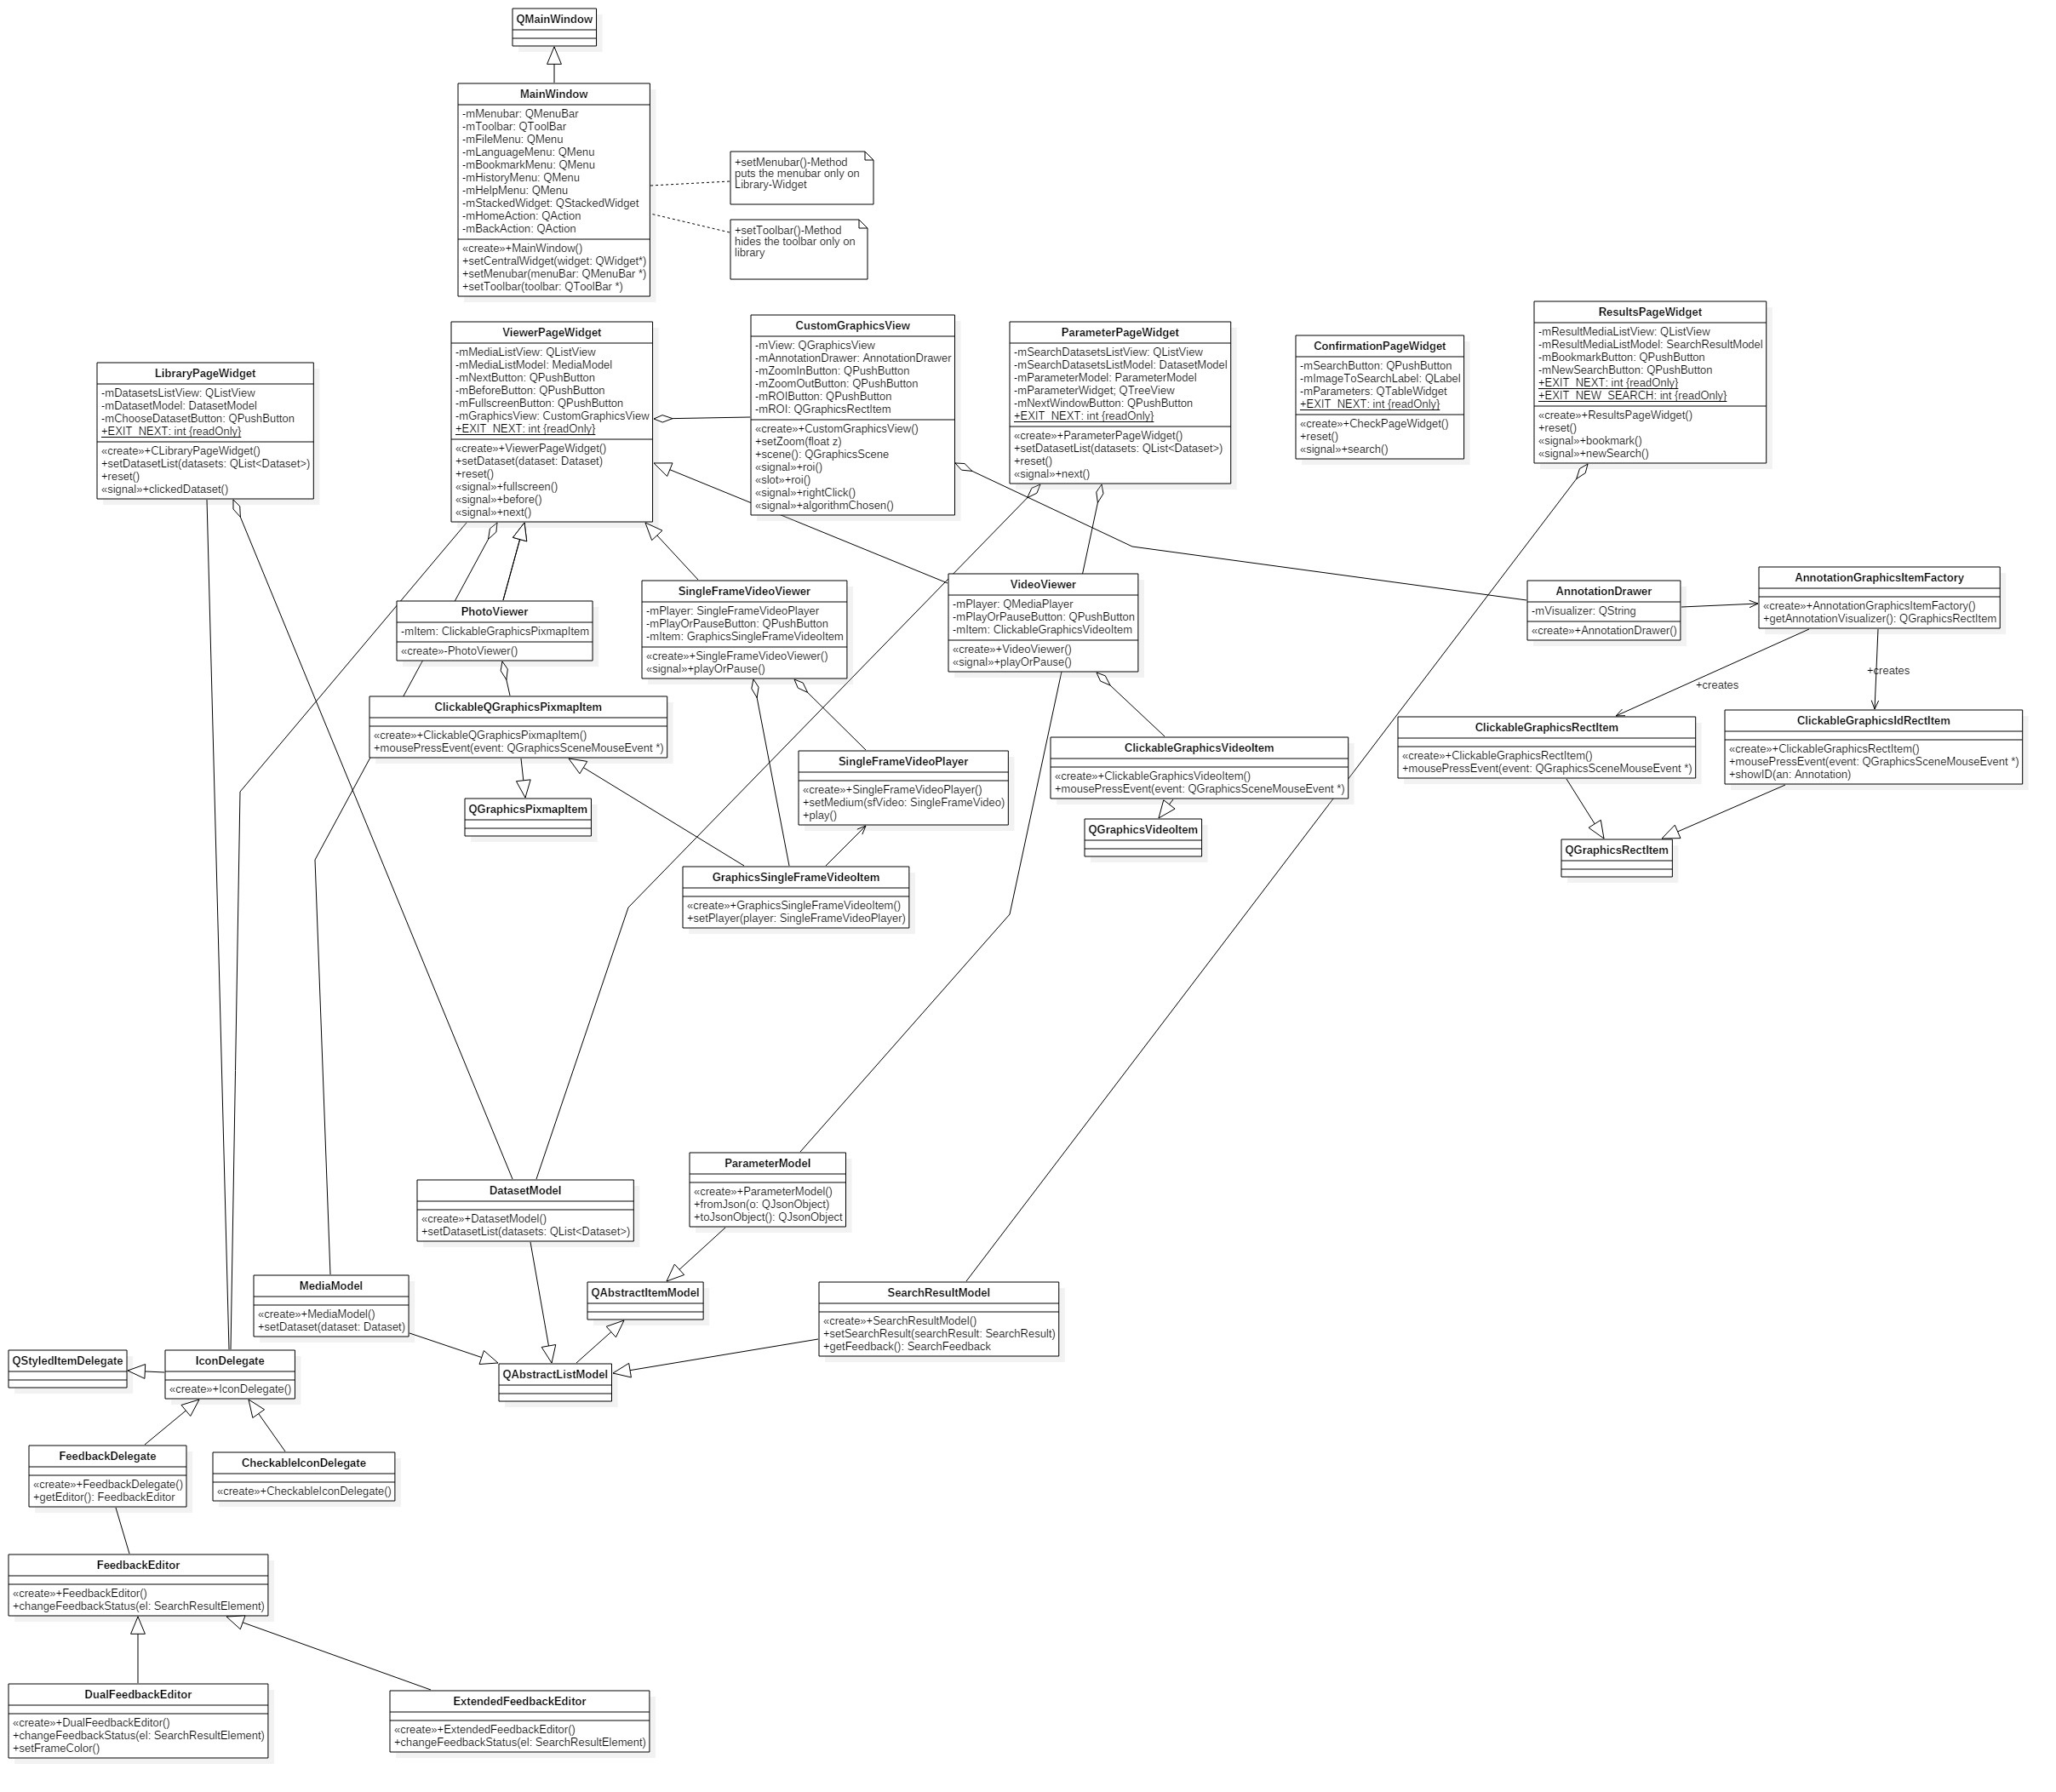
\includegraphics[width=1\linewidth]{img/Klassendiagramm/View}
\caption{View}
\label{fig:view}
\end{figure}


\subsection*{<<abstract>> PageWidget : public QWidget}
Ein PageWidget ist ein QWidget, das als eine Seite der grafischen Oberfläche im MainWindow dem Benutzer angezeigt wird. Die abstrakte Klasse PageWidget bietet dem erbenden Widget, das momentan im MainWindow angezeigt wird, die Möglichkeit ein PageWidget auszusuchen. Dieses wird dem Benutzer als nächstes angezeigt. Über den Stack des Navigators werden benötige Daten an das PageWidget übergeben.

\begin{figure}[H]
	\centering
	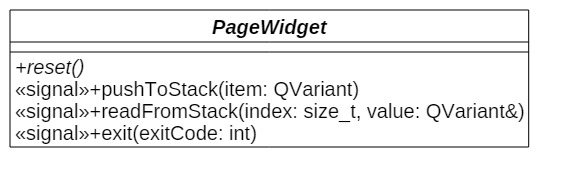
\includegraphics[scale=0.5]{img/Klassendiagramm/Klassen/View/PageWidget}
	\label{fig:pageWidget}
\end{figure}

\subsection*{MainWindow : public QMainWindow}
Die Klasse stellt das Hauptfenster des Programms dar, auf dem die weiteren Seiten als PageWidgets angezeigt werden.

\begin{figure}[H]
	\centering
	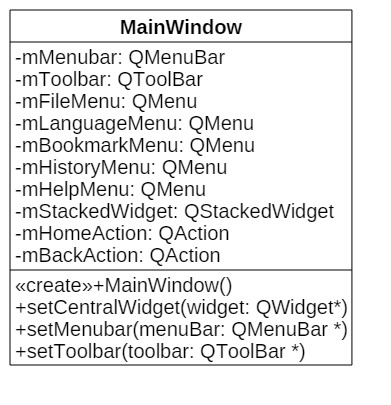
\includegraphics[scale=0.5]{img/Klassendiagramm/Klassen/View/MainWindow}
	\label{fig:mainWindow}
\end{figure}

Attribute
\begin{itemize}
	\item\textit{private QMenuBar mMenubar}
	Die Menubar, die in der Library gezeigt wird.   
	\item\textit{private QToolbar toolbar}
	Die Toolbar, die die Back- und Next-Buttons enthält.
	\item\textit{private QMenu mFileMenu}
	Das Dateimenü mit den Hauptfunktionen (Öffnen, Schließen, etc.)
	\item\textit{private QMenu mLanguageMenu}
	Das Menü mit den verfügbaren Sprachen.
	\item\textit{private QMenu mBookmarkMenu}
	Das Menü, mit dem man Lesezeicheneinträge öffnen kann.
	\item\textit{private QMenu mHistoryMenu}
	Das Menü, mit dem man die letzten Suchergebnisse öffnen kann.
	\item\textit{private QMenu mHelpMenu}
	Das Menü, mit dem man die Hilfe öffnen oder den About Dialog anzeigen kann.
	\item\textit{private QStackedWidget mStackedWidget}
	Das StackedWidget, in dem die PageWidgets gewechselt werden.
	\item\textit{private QAction mHomeAction}
	Aktion in der Toolbar, mit der man zum Hauptfenster zurückkommt.
	\item\textit{private QAction mBackAction}
	Aktion in der Toolbar, mit der man zu der vorherigen Seite zurückkommt.
\end{itemize}

Methoden
\begin{itemize}
	\item\textit{public MainWindow()} 
	Erzeugt ein neues MainWindow Objekt.
	\item\textit{public void setCentralWidget(QWidget *widget)} 
	Damit wird das aktuelle Widget gesetzt.
	\item\textit{public void setMenubar(QMenuBar *menuBar)} 
	Macht die MenuBar sichtbar oder unsichtbar.
	\item\textit{public void setToolbar(QToolBar *toolbar)} 
	Macht die Toolbar sichtbar oder unsichtbar.
\end{itemize}

\subsection*{LibraryPageWidget : public PageWidget}
Das PageWidget, in dem alle Datensätze dargestellt werden. Man kann einen Datensatz für die Suche auswählen. Durch den ChooseDataSetButton kann man auch einen Datensatz wählen, der nicht in der Datenbank liegt. 

\begin{figure}[H]
	\centering
	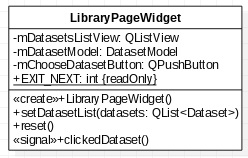
\includegraphics[scale=0.5]{img/Klassendiagramm/Klassen/View/LibraryPageWidget}
	\label{fig:libraryPageWidget}
\end{figure}

Attribute
\begin{itemize}
	\item\textit{private QListView mDatasetsListView} 
	Ein ListView zur Darstellung der Datensätze.
	\item\textit{private DatasetModel mDatasetModel}
	Ein DatasetModel, das die darzustellende Datensätze enthält.
	\item\textit{private QPushButton mChooseDatasetButton} 
	Ein PushButton, der einen FileDialog öffnet, um einen neuen Datensatz zu wählen.
	\item\textit{public int EXIT\_NEXT}
	Diese Konstante dient dazu, das nachfolgende PageWidget zu bestimmen.
\end{itemize}

Methoden
\begin{itemize}
	\item\textit{public LibraryPageWidget()} 
	Erzeugt ein neues LibraryPageWidget Objekt.
	\item\textit{public void setDatasetList(QList<Dataset> *datasets)} 
	Füllt ein DatasetModel mit den Datensätzen, die darzustellen sind.
	\item\textit{public void reset()} 
	Leert die Library.
	\item\textit{public signal clickedDataset()} 
	Ein Signal an den Controller, wenn auf einen Datensatz geklickt wurde.
\end{itemize}

\subsection*{ViewerPageWidget : public PageWidget}
Diese Klasse bildet die Basis für die PageWidgets, die den Inhalt eines Datensatzes in Form von Photoalbum oder Videoplayer darstellen.

\begin{figure}[H]
	\centering
	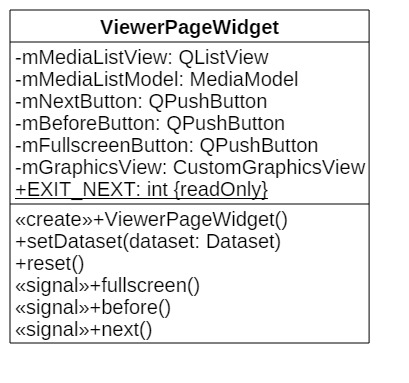
\includegraphics[scale=0.5]{img/Klassendiagramm/Klassen/View/ViewerPageWidget}
	\label{fig:viewerPageWidget}
\end{figure}

Attribute
\begin{itemize}
	\item\textit{private QListView mMediaListView}
	Ein ListView zur Darstellung der Media in dem Datensatz.
	\item\textit{private MediaModel mMediaListModel} 
	Ein MediaModel, das die darzustellende Media enthält.
	\item\textit{private QPushButton mNextButton}
	Button, mit dem man zum nächsten Medium zu wechseln. 
	\item\textit{private QPushButton MBeforeButton}
	Button, mit dem man zum vorherigen Medium zu wechseln.
	\item\textit{private QPushButton mFullscreenButton}
	Button für den Vollbild-Modus.
	\item\textit{private CustomGraphicsView mGraphicsView} 
	Die modifizierte GraphicsView, in der das gewählte Medium angezeigt bzw. abgespielt wird.  
	\item\textit{public int EXIT\_NEXT} 
	Diese Konstante dient dazu, das nachfolgende PageWidget zu bestimmen.     
\end{itemize}

\pagebreak
Methoden
\begin{itemize}
	\item\textit{public ViewerPageWidget()} 
	Erzeugt ein neues ViewerPageWidget Objekt.
	\item\textit{public void setDataset(Dataset *dataset)} 
	Füllt ein MediaModel mit den Media von einem gewählten Datensatz.
	\item\textit{public void reset()} 
	Leert den Viewer.
	\item\textit{public signal fullscreen()} 
	Ein Signal an den Controller, dass der FullscreenButton geklickt wurde.
	\item\textit{public signal before()} 
	Ein Signal an den Controller, dass der BeforeButton geklickt wurde.
	\item\textit{public signal next()}
	Ein Signal an den Controller, dass der NextButton geklickt wurde.
\end{itemize}

\subsection*{PhotoViewer : public ViewerPageWidget}
Seine Funktion ist das Darstellen der Bilder, die in einem Datensatz enthalten sind.

\begin{figure}[H]
	\centering
	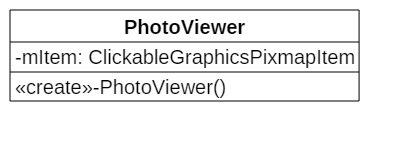
\includegraphics[scale=0.5]{img/Klassendiagramm/Klassen/View/PhotoViewer}
	\label{fig:photoVIewer}
\end{figure}

Attribute
\begin{itemize}
	\item\textit{private ClickableGraphicsPixmapItem mItem} 
	Ein GraphicsItem für die Darstellung des Bildes mit der Möglichkeit, Klicks abzufangen.    
\end{itemize}

Methoden
\begin{itemize}
	\item\textit{public PhotoViewer()}
	 Erzeugt ein neues PhotoViewer-Objekt.
\end{itemize}

\subsection*{ClickableQGraphicsPixmapItem : public QGraphicsPixmapItem}
Stellt das Bild dar, das bei CustomGraphicsView angezeigt wird und auf dem \glslink{Annotation}{Annotationen} gemacht werden können. Mit einem Rechtsklick kann man den \glslink{Suchalgorithmus}{Algorithmus} für die Suche wählen.

\begin{figure}[H]
	\centering
	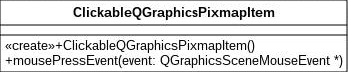
\includegraphics[scale=0.5]{img/Klassendiagramm/Klassen/View/ClickableQGraphicsPixmapItem}
	\label{fig:clickableQGraphicsPixmapItem}
\end{figure}

Methoden
\begin{itemize}
	\item\textit{public ClickableQGraphicsPixmapItem()} 
	Erzeugt ein neues ClickableQGraphicsPixmapItem-Objekt.
	\item\textit{public void mousePressEvent(QGraphicsSceneMouseEvent *event)} 
	Fängt den Rechtsklick des Benutzers ab und sendet die Position des Klicks als Signal an den Controller.
\end{itemize}

\subsection*{SingleFrameVideoViewer : public ViewerPageWidget}
Seine Funktion ist das Darstellen von Videos aus einem Datensatz, die in Form von Einzelbildern vorliegen.

\begin{figure}[H]
	\centering
	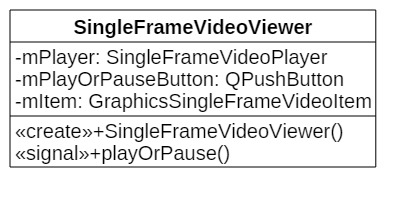
\includegraphics[scale=0.5]{img/Klassendiagramm/Klassen/View/SingleFrameVideoViewer}
	\label{fig:singleFrameVideoViewer}
\end{figure}

Attribute
\begin{itemize}
	\item\textit{private SingleFrameVideoPlayer mPlayer} 
	Ein SingleFrameVideoPlayer, der das Video abspielt. 
	\item\textit{private QPushButton mPlayOrPauseButton} 
	Ein Button, um das Video abzuspielen oder zu pausieren.
	\item\textit{private GraphicsSingleFrameVideoItem mItem} 
	Ein GraphicsItem, das ein SingleFrameVideo abspielt und ClickableQGraphicsPixmapItems benutzt.
\end{itemize}

Methoden
\begin{itemize}
	\item\textit{public SingleFrameVideoViewer()} 
	Erzeugt ein neues SingleFrameVideoViewer-Objekt.
	\item\textit{public void signa playOrPause()} 
	Ein Signal an den Controller, wenn der PlayOrPauseButton geklickt wurde.
\end{itemize} 

\subsection*{SingleFrameVideoPlayer} 
Eine Komponente des SingleFrameVideoViewer, die das Video in Form von Einzelbildern in dem GraphicsView anzeigt.

\begin{figure}[H]
	\centering
	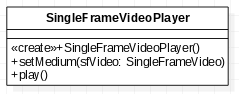
\includegraphics[scale=0.5]{img/Klassendiagramm/Klassen/View/SingleFrameVideoPlayer}
	\label{fig:singleFrameVideoPlayer}
\end{figure}

Methoden
\begin{itemize}
	\item\textit{public SingleFrameVideoPlayer()} 
	Erzeugt ein neues SingleFrameVideoPlayer-Objekt.
	\item\textit{public void setMedium(SingleFrameVideo sfVideo)} 
	Gibt dem Player ein Medium.
	\item\textit{public void play()} 
	Beginnt das Abspielen des Videos.
\end{itemize}

\subsection*{GraphicsSingleFrameVideoItem : public ClickableQGraphicsPixmapItem}
Stellt mithilfe des SingleFrameVideoPlayers ein Video aus Einzelbildern dar, wobei man Bereiche markieren, Annotationen auswählen und mit einem Rechtsklick den \glslink{Suchalgorithmus}{Algorithmus} wählen kann.

\begin{figure}[H]
	\centering
	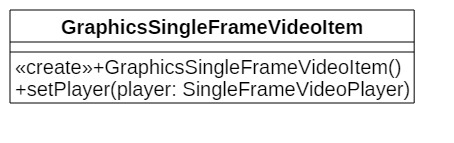
\includegraphics[scale=0.5]{img/Klassendiagramm/Klassen/View/GraphicsSingleFrameVideoItem}
	\label{fig:graphicsSingleFrameVideoItem}
\end{figure}

Methoden
\begin{itemize}
	\item\textit{public GraphicsSingleFrameVideoItem()} 
	Erzeugt ein neues GraphicsSingleFrameVideoItem-Objekt.
	\item\textit{public void setPlayer(CSingleFrameVideoPlayer player)} 
	Setzt den VideoPlayer für das Abspielen des Videos.
\end{itemize}

\subsection*{VideoViewer : public ViewerPageWidget}
Seine Funktion ist das Darstellen und Abspielen der Videos aus Videodateien, die in einem Datensatz enthalten sind.

\begin{figure}[H]
	\centering
	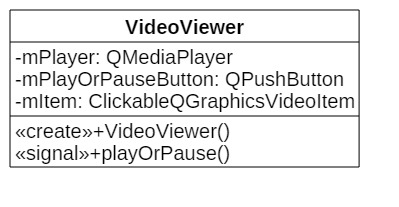
\includegraphics[scale=0.5]{img/Klassendiagramm/Klassen/View/VideoViewer}
	\label{fig:videoViewer}
\end{figure}

Attribute
\begin{itemize}
	\item\textit{private QMediaPlayer mPlayer} 
	Ein MediaPlayer, der das Video abspielt. 
	\item\textit{private QPushButton mPlayOrPauseButton} 
	Ein Button, um das Video abzuspielen oder zu pausieren.
	\item\textit{private ClickableGraphicsVideoItem mItem} 
	Ein GraphicsItem für die Darstellung des Videos mit der Möglichkeit, Klicks abzufangen.     
\end{itemize}
\pagebreak
Methoden
\begin{itemize}
	\item\textit{public VideoViewer()} 
	Erzeugt ein neues VideoViewer-Objekt.
	\item\textit{public signal playOrPause()} 
	EIn Signal an den Controller, wenn der PlayOrPauseButton geklickt wurde.
\end{itemize} 

\subsection*{ClickableQGraphicsVideoItem : public QGraphicsVideoItem}
Stellt das Video dar, das bei CustomGraphicsView angezeigt wird und auf dem man Bereiche markieren und \glslink{Annotation}{Annotationen} auswählen kann. Mit einem Rechtsklick kann man den \glslink{Suchalgorithmus}{Algorithmus} für die Suche wählen.

\begin{figure}[H]
	\centering
	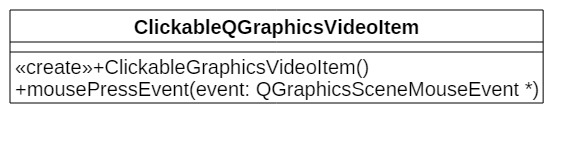
\includegraphics[scale=0.5]{img/Klassendiagramm/Klassen/View/ClickableQGraphicsVideoItem}
	\label{fig:clickableQGraphicsVideoItem}
\end{figure}

Methoden
\begin{itemize}
	\item\textit{public ClickableQGraphicsVideoItem()} 
	Erzeugt ein neues ClickableQGraphicsVideoItem-Objekt.
	\item\textit{public void mousePressEvent(QGraphicsSceneMouseEvent *event)} 
	Fängt den Rechtsklick des Benutzers ab, bestimmt den Frame und die Position des Klicks und sendet ein Signal an den Controller.
\end{itemize}

\subsection*{CustomGraphicsView}
Diese Klasse benutzt ein QGraphicsView um ein Bild darzustellen und einen AnnotationDrawer um die \glslink{Annotation}{Annotationen}, die zum Bild gehören, darzustellen. Außerdem fügt er die Möglichkeit hinzu, die Größe des Bildes durch die ZoomIn- und ZoomOutButtons zu verändern und eine \gls{ROI}(\enquote{region of interest}) zu zeichnen, nach der dann gesucht werden kann. Hier werden auch die Klicks des Benutzers abgefangen und das Menü mit den \glslink{Suchalgorithmus}{Algorithmen} angezeigt.

\begin{figure}[H]
	\centering
	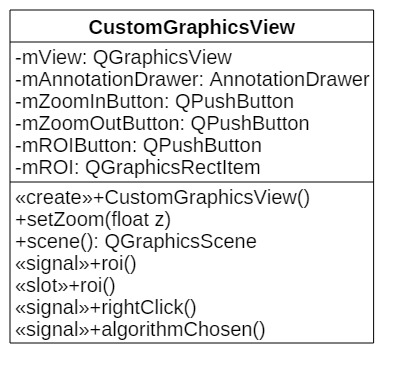
\includegraphics[scale=0.5]{img/Klassendiagramm/Klassen/View/CustomGraphicsView}
	\label{fig:customGraphicsView}
\end{figure}

Attribute
\begin{itemize}
	\item\textit{private QGraphicsView mView} 
	Ein GraphicsView, in der das Medium angezeigt wird. 
	\item\textit{private AnnotationDrawer mAnnotationDrawer} 
	Ein AnnotationDrawer, der die \glslink{Annotation}{Annotationen} des Bildes/Frames hinzufügt. 
	\item\textit{private QPushButton mZoomInButton} 
	Ein PushButton für die ZoomIn Funktion. 
	\item\textit{private QPushButton mZoomOutButton} 
	Ein PushButton für die ZoomOut Funktion.
	\item\textit{private QPushButton mROIButton} 
	Ein PushButton für das Einzeichnen einer \glslink{ROI}{\enquote{region of interest}}.
	\item\textit{private QGraphicsRectItem mROI} 
	Ein QGraphicsRectItem, der die vom Benutzer gezeichnete \glslink{ROI}{\enquote{region of interest}} darstellt.
\end{itemize}

Methoden
\begin{itemize}
	\item\textit{public CustomGraphicsView()} 
	Erzeugt ein neues CustomGraphicsView-Objekt.
	\item\textit{public void setZoom(float z)} 
	Setzt die Größe des Bildes/Frames.
	\item\textit{public QGraphicsScene scene()} 
	Erzeugt ein QGraphicsScene, in dem die Media gezeigt werden.
	\item\textit{public signal roi()} 
	Ein Signal, wenn der \glslink{ROI}{ROIButton} geklickt wurde.
	\item\textit{public slot void roi()} 
	Fängt das Signal roi ab und wartet darauf, dass der Benutzer ein Rechteck zeichnet.
	\item\textit{public signal rightClick()} 
	Ein Signal mit Positionsinformationen für den Controller, wenn ein Rechtsklick erfolgt. 
	\item\textit{public signal algorithmChosen()} 
	Ein Signal an den Controller mit der Information, welcher \glslink{Suchalgorithmus}{Algorithmus} gewählt wurde.
\end{itemize}

\subsection*{AnnotationDrawer}
Diese Klasse besitzt einen String, der den Typ der \gls{Annotation} bestimmt. Der AnnotationDrawer benutzt die AnnotationGraphicsItemFactory, um ein korrespondierendes ClickableGraphicsItem zu erzeugen, das er im CustomGraphicsView anzeigt.

\begin{figure}[H]
	\centering
	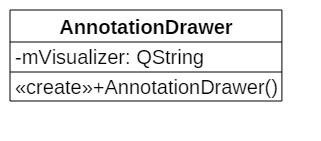
\includegraphics[scale=0.5]{img/Klassendiagramm/Klassen/View/AnnotationDrawer}
	\label{fig:annotationDrawer}
\end{figure}

Attribute
\begin{itemize}
	\item\textit{private QString mVisualizer} 
	Der Typ der \gls{Annotation}.   
\end{itemize}

Methoden
\begin{itemize}
	\item\textit{public AnnotationDrawer()} 
	Erzeugt ein neues AnnotationDrawer-Objekt.
\end{itemize}
  
\subsection*{AnnotationGraphicsItemFactory}
Das ist eine Fabrik-Klasse, die unterschiedliche ClickableGraphicsItems bildet, damit man die \glslink{Annotation}{Annotationen}, abhängig von deren Typ, durch den AnnotationDrawer darstellen kann.

\begin{figure}[H]
	\centering
	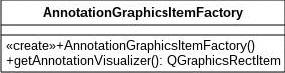
\includegraphics[scale=0.5]{img/Klassendiagramm/Klassen/View/AnnotationGraphicsItemFactory}
	\label{fig:annotationGraphicsItemFactory}
\end{figure}

Methoden
\begin{itemize}
	\item\textit{public AnnotationGraphicsItemFactory()} 
	Erzeugt ein neues AnnotationGraphicsItemFactory-Objekt.
	\item\textit{public QGraphicsRectItem getAnnotationVisualizer()} 
	Erzeugt ein QGraphicsItem, dem Visualizer entsprechend.
\end{itemize}
 
\subsection*{ClickableGraphicsRectItem : public QGraphicsRectItem}
Diese Klasse fügt die Möglichkeit hinzu, auf dieses Item klicken zu können.

\begin{figure}[H]
	\centering
	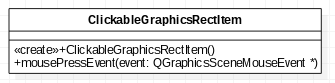
\includegraphics[scale=0.5]{img/Klassendiagramm/Klassen/View/ClickableGraphicsRectItem}
	\label{fig:clickableGraphicsRectItem}
\end{figure}

Methoden
\begin{itemize}
	\item\textit{public ClickableGraphicsRectItem()}
	Erzeugt ein neues ClickableGraphicsRectItem-Objekt.
	\item\textit{public void mousePressEvent(QGraphicsSceneMouseEvent *event)}
	Fängt die Bewegung der Maus nach einem Klick ab.
\end{itemize}

\subsection*{ClickableGraphicsIdRectItem : public QGraphicsRectItem}
Diese Klasse fügt die Möglichkeit hinzu, auf dieses Item klicken zu können, und zeigt die Id der \gls{Annotation}.

\begin{figure}[H]
	\centering
	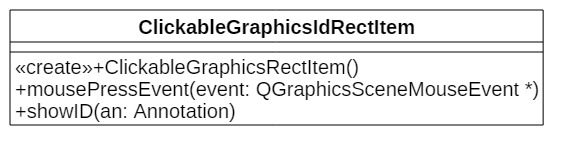
\includegraphics[scale=0.5]{img/Klassendiagramm/Klassen/View/ClickableGraphicsIdRectItem}
	\label{fig:clickableGraphicsIdRectItem}
\end{figure}

Methoden
\begin{itemize}
	\item\textit{public ClickableGraphicsIdRectItem()}
	Erzeugt ein neues ClickableGraphicsIdRectItem-Objekt.
	\item\textit{public void mousePressEvent(QGraphicsSceneMouseEvent *event)}
	Fängt die Bewegung der Maus nach einem Klick ab.
	\item\textit{public void showID(Annotation *an)}
	Zeigt die ID der \gls{Annotation} an.
\end{itemize}

\subsection*{ParameterPageWidget : public PageWidget}
Das ist das PageWidget, in dem die Parameter für den gewählten \gls{Suchalgorithmus} angezeigt und bestimmt werden. Außerdem werden die Datensätze, in denen gesucht wird, bestimmt. Dann kann man zu ConfirmationPageWidget fortsetzen.

\begin{figure}[H]
	\centering
	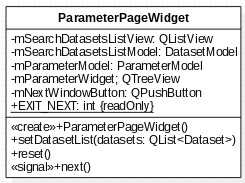
\includegraphics[scale=0.5]{img/Klassendiagramm/Klassen/View/ParameterPageWidget}
	\label{fig:parameterPageWidget}
\end{figure}

Attribute
\begin{itemize}
	\item\textit{private QListView mSearchDatasetListView}
	Ein ListView zur Darstellung der Datensätze, in denen gesucht werden kann.
	\item\textit{private DatasetModel mSearchDatasetListModel}
	Ein DatasetModel, das die darzustellende Datensätze enthält.
	\item\textit{private ParameterModel mParameterModel}
	Ein ParameterModel, das die darzustellende Parameter enthält.
	\item\textit{private QTreeView mParameterWidget}
	Ein TreeView zur Darestellung der Parameter.
	\item\textit{private QPushButton mNextWindowButton}
	Ein Button, mit dem zum nächsten Fenster gewechselt wird.
	\item\textit{public int EXIT\_NEXT} 
	Diese Konstante dient dazu, das nachfolgende PageWidget zu bestimmen.    
\end{itemize}

Methoden
\begin{itemize}
	\item\textit{public ParameterPageWidget()}
	Erzeugt ein ParameterPageWidget-Objekt.
	\item\textit{public void setDatasetList(QList<Dataset> *datasets)}
	Füllt ein DatasetModel mit den Datensätzen, die darzustellen sind.
	\item\textit{public void reset()}
	Leert das ParameterPageWidget.
	\item\textit{public signal next()}
	Ein Signal an den Controller, wenn das mNextWindowButton gefordert wird. 
\end{itemize}

\subsection*{ConfirmationPageWidget : public PageWidget}
Das PageWidget, in dem die Suchvorlage und alle Parameter angezeigt werden, sodass der Benutzer diese überprüfen kann. Mit dem SearchButton wird die Suche gestartet.

\begin{figure}[H]
	\centering
	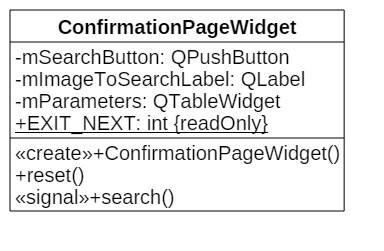
\includegraphics[scale=0.5]{img/Klassendiagramm/Klassen/View/ConfirmationPageWidget}
	\label{fig:confirmationPageWidget}
\end{figure}

Attribute
\begin{itemize}
	\item\textit{private QPushButton mSearchButton}
	Ein Button, mit dem man die Suche startet.
	\item\textit{private QLabel mImageToSearchLabel}
	Das Bild, auf der man die Suche durchführt.
	\item\textit{private QTableWidget mParameters}
	Eine Tabelle, die die gewählte Parameter anzeigt.
	\item\textit{public int EXIT\_NEXT} 
	Diese Konstante dient dazu, das nachfolgende PageWidget zu bestimmen. 
\end{itemize}

Methoden
\begin{itemize}
	\item\textit{public ConfirmationPageWidget()}
	Erzeugt ein ConfirmationPageWidget-Objekt.
	\item\textit{public void reset()}
	Leert das ConfirmationPageWidget. 
	\item\textit{public signal search()}
	Ein Signal an den Controller, wenn man das mSearchButton klickt.
\end{itemize}

\subsection*{ResultsPageWidget : public PageWidget}
Das ist das PageWidget, in dem die Ergebnisse der Suche dargestellt werden. Man kann die Suche speichern und bewerten. Nach der Bewertung kann erneut gesucht werden.

\begin{figure}[H]
	\centering
	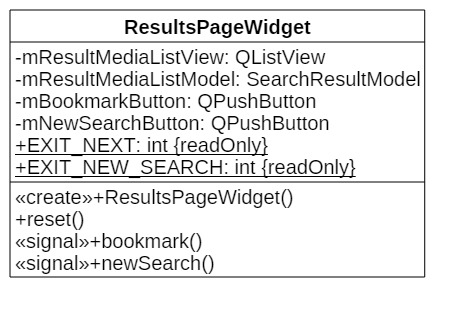
\includegraphics[scale=0.5]{img/Klassendiagramm/Klassen/View/ResultsPageWidget}
	\label{fig:resultsPageWidget}
\end{figure}
\pagebreak
Attribute
\begin{itemize}
	\item\textit{private QListView mResultMediaListView}
	Ein ListView zur Darstellung der Ergebnisse von der Suche.
	\item\textit{private SearchResultModel mResultMediaListModel}
	Ein SearchResultModel, das die darzustellende Ergebnisse enthält.
	\item\textit{private QPushButton mBookmarkButton()}
	Ein Button, mit dem man ein Bookmark setzt.
	\item\textit{private QPushButton mNewSearchButton}
	Ein Button, mit dem man eine neue Suche startet.
	\item\textit{public int EXIT\_NEXT}  
	Diese Konstante dient dazu, das nachfolgende PageWidget zu bestimmen.
	\item\textit{public int EXIT\_NEW\_SEARCH}
	Diese Konstante dient dazu, das nachfolgende PageWidget zu bestimmen.  
\end{itemize}

Methoden
\begin{itemize}
	\item\textit{public ResultsPageWidget()}
	Erzeugt ein ResultsPageWidget-Objekt.
	\item\textit{public void reset()}
	Leert das ResultsPageWidget.
	\item\textit{public signal bookmark()}
	Ein Signal an den Controller, wenn man das mBookmarkButton klickt.
	\item\textit{public signal newSearch()}
	Ein Signal an den Controller, wenn man das mNewSearchButton klickt.
\end{itemize}

\subsection*{SearchResultModel : public QAbstractListModel}
Bildet die Grundlage für die Anzeige der Ergebnisse im ListView.

\begin{figure}[H]
	\centering
	\includegraphics[scale=0.5]{img/Klassendiagramm/Klassen/View/SearchResultModel}
	\label{fig:searchResultModel}
\end{figure}

Methoden
\begin{itemize}
	\item\textit{public SearchResultModel()}
	Erzeugt ein SearchResultModel-Objekt.
	\item\textit{public void setSearchResult(Searchresult *searchResult)}
	Füllt ein SearchResultModel mit den Ergebnissen, die darzustellen sind.
	\item\textit{public SearchFeedback getFeedback()}
	Zeigt das Feedback für jedes Ergebnis an.
\end{itemize}

\subsection*{ParameterModel : public QAbstractItemModel}
Bildet die Grundlage für die Anzeige der Parameter eines QJsonObjects im ListView.

\begin{figure}[H]
	\centering
	\includegraphics[scale=0.5]{img/Klassendiagramm/Klassen/View/ParameterModel}
	\label{fig:parameterModel}
\end{figure}

Methoden
\begin{itemize}
	\item\textit{public ParameterModel()}
	Erzeugt ein ParameterModel-Objekt.
	\item\textit{public void fromJson(QJsonObject *o)}
	Erhält die Parameter von einem Json-Objekt.
	\item\textit{public QJsonObject toJsonObject()}
	Schreibt die Parameter in ein Json-Objekt.
\end{itemize}

\subsection*{DatasetModel : public QAbstractListModel}
Bildet die Grundlage für die Anzeige der Datensätze im ListView bei LibraryPageWidget und ParameterPageWidget.

\begin{figure}[H]
	\centering
	\includegraphics[scale=0.5]{img/Klassendiagramm/Klassen/View/DatasetModel}
	\label{fig:datasetModel}
\end{figure}

Methoden
\begin{itemize}
	\item\textit{public DatasetModel()}
	Erzeugt ein DatasetModel-Objekt.
	\item\textit{public void setDatasetList(QList<Dataset> *datasets)}
	Füllt ein DatasetModel mit den Datensätzen, die darzustellen sind.
\end{itemize}

\subsection*{MediaModel : public QAbstractListModel}
Bildet die Grundlage für die Anzeige der Media-Dateien im ListView bei ViewerPageWidget.

\begin{figure}[H]
	\centering
	\includegraphics[scale=0.5]{img/Klassendiagramm/Klassen/View/MediaModel}
	\label{fig:mediaModel}
\end{figure}

Methoden
\begin{itemize}
	\item\textit{public MediaModel()}
	Erzeugt ein MediaModel-Objekt.
	\item\textit{public void setDataset(Dataset *dataset)}
	Füllt ein MediaModel mit den Medien eines gewählten Datensatzes.
\end{itemize}

\subsection*{IconDelegate : public QStyledItemDelegate}
Diese Klasse ist ein anklickbares IconDelegate, das aus einem Bild und darunter Text besteht. Diese nutzt man, um die Datensätze in LibraryPageWidget, ViewerPageWidget darzustellen und herauszufinden, welcher von denen ausgewählt wurde.

\begin{figure}[H]
	\centering
	\includegraphics[scale=0.5]{img/Klassendiagramm/Klassen/View/IconDelegate}
	\label{fig:iconDelegate}
\end{figure}
\pagebreak
Methoden
\begin{itemize}
	\item\textit{public IconDelegate()}
	Erzeugt ein IconDelegate-Objekt.
\end{itemize}

\subsection*{CheckableIconDelegate : public IconDelegate}
Diese Klasse fügt eine Checkbox hinzu. Damit werden die Datensätze im ParameterPageWidget dargestellt und man bekommt die Information, in welchen gesucht wird.

\begin{figure}[H]
	\centering
	\includegraphics[scale=0.5]{img/Klassendiagramm/Klassen/View/CheckableIconDelegate}
	\label{fig:checkableIconDelegate}
\end{figure}

Methoden
\begin{itemize}
	\item\textit{public CheckableIconDelegate()}
	Erzeugt ein CheckableIconDelegate-Objekt.
\end{itemize} 

\subsection*{FeedbackDelegate : public IconDelegate}
Die Klasse kann einen FeedbackEditor benutzen, um Feedback zu bekommen. Man nutzt diese Klasse, um die Resultate der Suche in ResultsPageWidget darzustellen, mit der Option, Feedback zu bekommen. 

\begin{figure}[H]
	\centering
	\includegraphics[scale=0.5]{img/Klassendiagramm/Klassen/View/FeedbackDelegate}
	\label{fig:feedbackDelegate}
\end{figure}

Methoden
\begin{itemize}
	\item\textit{public FeedbackDelegate()}
	Erzeugt ein FeedbackDelegate-Objekt.
	\item\textit{public FeedbackEditor getEditor()}
	Erzeugt einen FeedbackEditor.
\end{itemize}

\subsection*{FeedbackEditor}
Diese Klasse stellt Feedback graphisch dar und bekommt die Werte des Feedbacks abhängig vom Typ des Feedbacks.

\begin{figure}[H]
	\centering
	\includegraphics[scale=0.5]{img/Klassendiagramm/Klassen/View/FeedbackEditor}
	\label{fig:feedbackEditor}
\end{figure}

Methoden
\begin{itemize}
	\item\textit{public FeedbackEditor()}
	Erzeugt ein FeedbackEditor-Objekt.
	\item\textit{public void changeFeedbackStatus(SearchResultElement *el)}
	Verändert das Feedback des zugehörigen Suchelements.
\end{itemize}

\subsection*{DualFeedbackEditor : public FeedbackEditor}
Stellt duales Feedback (positiv, neutral, negativ) dar.

\begin{figure}[H]
	\centering
	\includegraphics[scale=0.5]{img/Klassendiagramm/Klassen/View/DualFeedbackEditor}
	\label{fig:dualFeedbackEditor}
\end{figure}

Methoden
\begin{itemize}
	\item\textit{public DualFeedbackEditor()}
	Erzeugt ein DualFeedbackEditor-Objekt.
	\item\textit{public void changeFeedbackStatus(SearchResultElement *el)}
	Verändert das Feedback des zugehörigen Suchelements.
	\item\textit{public void setFrameColor()}
	Setzt den Bildrahmen auf die Farbe, die das Feedback zurückgibt. 
\end{itemize}

\subsection*{ExtendedFeedbackEditor : public FeedbackEditor}
Stellt erweitertes Feedback (Werte von 1 bis 10) dar.

\begin{figure}[H]
	\centering
	\includegraphics[scale=0.5]{img/Klassendiagramm/Klassen/View/ExtendedFeedbackEditor}
	\label{fig:ExtendedFeedbackEditor}
\end{figure}

Methoden
\begin{itemize}
	\item\textit{public ExtendedFeedbackEditor()}
	Erzeugt ein ExtendedFeedbackEditor-Objekt.
	\item\textit{public void changeFeedbackStatus(SearchResultElement *el)}
	Verändert das Feedback des zugehörigen Suchelements.
\end{itemize}

\pagebreak

\subsection{Controller}

Dieses Diagramm zeigt alle Klassen des Controllers. Die zugehörigen Attribute und Methoden werden im Folgenden beschrieben.

\begin{figure}[H]
\includegraphics[width=1\linewidth]{img/Klassendiagramm/Controller}
\caption{Controller}
\label{fig:controller}
\end{figure}

\pagebreak

\subsection*{MainControl}
MainControl ist der Einstiegspunkt des Programms und verwaltet die Manager-Klassen sowie den Navigator. Insbesondere erstellt MainControl die PageWidgets und registriert sie beim Navigator.
Da die Manager und der Navigator nicht direkt kommunizieren, verbindet MainControl ihre Signals und Slots.

\begin{figure}[H]
\centering
\includegraphics[scale=0.5]{img/Klassendiagramm/Klassen/Controller/MainControl}
\label{fig:mainControl}
\end{figure}

\subsection*{Navigator}
Der Navigator ist in der Lage, das aktuell im MainWindow angezeigte PageWidget durch ein anderes zu ersetzen. Des weiteren ist der Navigator für den Austausch von Daten zwischen den PageWidgets verantwortlich.

\begin{figure}[H]
\centering
\includegraphics[scale=0.5]{img/Klassendiagramm/Klassen/Controller/Navigator}
\label{fig:navigator}
\end{figure}

\subsection*{SearchManager}
Der SearchManager startet einen \glslink{Suchalgorithmus}{Algorithmus} in einem neuen Thread und leitet mögliche Informationen zum Fortschritt der Suche an das ResultsPageWidget weiter.

\begin{figure}[H]
\centering
\includegraphics[scale=0.5]{img/Klassendiagramm/Klassen/Controller/SearchManager}
\label{fig:searchManager}
\end{figure}

\subsection*{SearchResultManager}
Der SearchResultManager besitzt ein SearchResult und benachrichtigt das ResultsPageWidget über neue Suchergebnisse. Suchergebnisse können einzeln während der laufenden Suche hinzugefügt werden.

\begin{figure}[H]
\centering
\includegraphics[scale=0.5]{img/Klassendiagramm/Klassen/Controller/SearchResultManager}
\label{fig:searchResultManager}
\end{figure}

\subsection*{MainWindowManager}
Der MainWindowManager stellt die Bookmarks und Chronikeinträge dem MainWindow zur Verfügung und gibt bekannt, welches Bookmark im MainWindow zuletzt ausgewählt wurde.

\begin{figure}[H]
\centering
\includegraphics[scale=0.5]{img/Klassendiagramm/Klassen/Controller/MainWindowManager}
\label{fig:mainWindowManager}
\end{figure}

\subsection*{BookmarkManager}
Der BookmarkManager besitzt 2 Listen für die Chronik und die vom Benutzer erstellten Bookmarks. Einträge für diese BookmarkLists werden über den BookmarkManager hinzugefügt und abgefragt.

\begin{figure}[H]
\centering
\includegraphics[scale=0.5]{img/Klassendiagramm/Klassen/Controller/BookmarkManager}
\label{fig:bookmarkManager}
\end{figure}

\subsection*{PageStackFrame}

\begin{figure}[H]
\centering
\includegraphics[scale=0.5]{img/Klassendiagramm/Klassen/Controller/PageStackFrame}
\label{fig:pageStackFrame}
\end{figure}

\subsection*{PageRegistration}

\begin{figure}[H]
\centering
\includegraphics[scale=0.5]{img/Klassendiagramm/Klassen/Controller/PageRegistration}
\label{fig:pageRegistration}
\end{figure}

\subsection*{<<enumeration>> PageType}
PageWidgets lassen sich beim Navigator mit einem PageType registrieren, welcher fortan zur Referenzierung dieses PageWidgets dient.

\begin{figure}[H]
\centering
\includegraphics[scale=0.5]{img/Klassendiagramm/Klassen/Controller/PageType}
\label{fig:pageType}
\end{figure}

\section{Sequenzdiagramme}
\begin{figure}[H]
\centering
\includegraphics[width=\linewidth]{img/Sequenzdiagramme/Navigation(short)}
\label{fig:navigation}
\end{figure}

\begin{figure}[H]
\centering
\includegraphics[width=\linewidth]{img/Sequenzdiagramme/Seitenwechsel}
\label{fig:seitenwechsel}
\end{figure}

\begin{figure}[H]
\centering
\includegraphics[width=\linewidth]{img/Sequenzdiagramme/SucheStarten}
\label{fig:sucheStarten}
\end{figure}

\begin{figure}[H]
\centering
\includegraphics[width=\linewidth]{img/Sequenzdiagramme/SucheTerminieren}
\label{fig:sucheTerminieren}
\end{figure}

\begin{figure}[H]
\centering
\includegraphics[width=\linewidth]{img/Sequenzdiagramme/SuchergebnisSpeichern}
\label{fig:suchergebnisSpeichern}
\end{figure}

\section{Entwurfsdaten}
\begin{itemize}
\item Die Parameter werden in Form von Name und Standardwert im Json Format gespeichert.
\item Die Annotationen sind in einer .persontracks Datei, die im Datensatz vorhanden ist, hinterlegt. In dieser Datei sind für jedes Medium die Anzahl der Annotationen und ihre jeweiligen Annotationsdaten gespeichert: Position im Medium, Größe, ID und Typ der Annotation.
\item Die Framerate für ein SingleFrameVideo wird in einer cobab\_config.json Datei gespeichert.
\item Die CoBaB Einstellungsdaten werden mithilfe von QSettings verwaltet.
\end{itemize}

\section{Anhang}
\input{include/anhang.tex}

\section{Glossar}

\end{document}
